\documentclass[]{article}
\usepackage{lmodern}
\usepackage{amssymb,amsmath}
\usepackage{ifxetex,ifluatex}
\usepackage{fixltx2e} % provides \textsubscript
\ifnum 0\ifxetex 1\fi\ifluatex 1\fi=0 % if pdftex
  \usepackage[T1]{fontenc}
  \usepackage[utf8]{inputenc}
\else % if luatex or xelatex
  \ifxetex
    \usepackage{mathspec}
  \else
    \usepackage{fontspec}
  \fi
  \defaultfontfeatures{Ligatures=TeX,Scale=MatchLowercase}
\fi
% use upquote if available, for straight quotes in verbatim environments
\IfFileExists{upquote.sty}{\usepackage{upquote}}{}
% use microtype if available
\IfFileExists{microtype.sty}{%
\usepackage{microtype}
\UseMicrotypeSet[protrusion]{basicmath} % disable protrusion for tt fonts
}{}
\usepackage[margin=1in]{geometry}
\usepackage{hyperref}
\PassOptionsToPackage{usenames,dvipsnames}{color} % color is loaded by hyperref
\hypersetup{unicode=true,
            pdftitle={Differential Expression Analysis of mRNA-seq Data from Single Cell and Circulating Tumor Cells},
            pdfauthor={Ugne Jankauskaite},
            colorlinks=true,
            linkcolor=Maroon,
            citecolor=Blue,
            urlcolor=blue,
            breaklinks=true}
\urlstyle{same}  % don't use monospace font for urls
\usepackage{color}
\usepackage{fancyvrb}
\newcommand{\VerbBar}{|}
\newcommand{\VERB}{\Verb[commandchars=\\\{\}]}
\DefineVerbatimEnvironment{Highlighting}{Verbatim}{commandchars=\\\{\}}
% Add ',fontsize=\small' for more characters per line
\usepackage{framed}
\definecolor{shadecolor}{RGB}{248,248,248}
\newenvironment{Shaded}{\begin{snugshade}}{\end{snugshade}}
\newcommand{\KeywordTok}[1]{\textcolor[rgb]{0.13,0.29,0.53}{\textbf{#1}}}
\newcommand{\DataTypeTok}[1]{\textcolor[rgb]{0.13,0.29,0.53}{#1}}
\newcommand{\DecValTok}[1]{\textcolor[rgb]{0.00,0.00,0.81}{#1}}
\newcommand{\BaseNTok}[1]{\textcolor[rgb]{0.00,0.00,0.81}{#1}}
\newcommand{\FloatTok}[1]{\textcolor[rgb]{0.00,0.00,0.81}{#1}}
\newcommand{\ConstantTok}[1]{\textcolor[rgb]{0.00,0.00,0.00}{#1}}
\newcommand{\CharTok}[1]{\textcolor[rgb]{0.31,0.60,0.02}{#1}}
\newcommand{\SpecialCharTok}[1]{\textcolor[rgb]{0.00,0.00,0.00}{#1}}
\newcommand{\StringTok}[1]{\textcolor[rgb]{0.31,0.60,0.02}{#1}}
\newcommand{\VerbatimStringTok}[1]{\textcolor[rgb]{0.31,0.60,0.02}{#1}}
\newcommand{\SpecialStringTok}[1]{\textcolor[rgb]{0.31,0.60,0.02}{#1}}
\newcommand{\ImportTok}[1]{#1}
\newcommand{\CommentTok}[1]{\textcolor[rgb]{0.56,0.35,0.01}{\textit{#1}}}
\newcommand{\DocumentationTok}[1]{\textcolor[rgb]{0.56,0.35,0.01}{\textbf{\textit{#1}}}}
\newcommand{\AnnotationTok}[1]{\textcolor[rgb]{0.56,0.35,0.01}{\textbf{\textit{#1}}}}
\newcommand{\CommentVarTok}[1]{\textcolor[rgb]{0.56,0.35,0.01}{\textbf{\textit{#1}}}}
\newcommand{\OtherTok}[1]{\textcolor[rgb]{0.56,0.35,0.01}{#1}}
\newcommand{\FunctionTok}[1]{\textcolor[rgb]{0.00,0.00,0.00}{#1}}
\newcommand{\VariableTok}[1]{\textcolor[rgb]{0.00,0.00,0.00}{#1}}
\newcommand{\ControlFlowTok}[1]{\textcolor[rgb]{0.13,0.29,0.53}{\textbf{#1}}}
\newcommand{\OperatorTok}[1]{\textcolor[rgb]{0.81,0.36,0.00}{\textbf{#1}}}
\newcommand{\BuiltInTok}[1]{#1}
\newcommand{\ExtensionTok}[1]{#1}
\newcommand{\PreprocessorTok}[1]{\textcolor[rgb]{0.56,0.35,0.01}{\textit{#1}}}
\newcommand{\AttributeTok}[1]{\textcolor[rgb]{0.77,0.63,0.00}{#1}}
\newcommand{\RegionMarkerTok}[1]{#1}
\newcommand{\InformationTok}[1]{\textcolor[rgb]{0.56,0.35,0.01}{\textbf{\textit{#1}}}}
\newcommand{\WarningTok}[1]{\textcolor[rgb]{0.56,0.35,0.01}{\textbf{\textit{#1}}}}
\newcommand{\AlertTok}[1]{\textcolor[rgb]{0.94,0.16,0.16}{#1}}
\newcommand{\ErrorTok}[1]{\textcolor[rgb]{0.64,0.00,0.00}{\textbf{#1}}}
\newcommand{\NormalTok}[1]{#1}
\usepackage{graphicx,grffile}
\makeatletter
\def\maxwidth{\ifdim\Gin@nat@width>\linewidth\linewidth\else\Gin@nat@width\fi}
\def\maxheight{\ifdim\Gin@nat@height>\textheight\textheight\else\Gin@nat@height\fi}
\makeatother
% Scale images if necessary, so that they will not overflow the page
% margins by default, and it is still possible to overwrite the defaults
% using explicit options in \includegraphics[width, height, ...]{}
\setkeys{Gin}{width=\maxwidth,height=\maxheight,keepaspectratio}
\IfFileExists{parskip.sty}{%
\usepackage{parskip}
}{% else
\setlength{\parindent}{0pt}
\setlength{\parskip}{6pt plus 2pt minus 1pt}
}
\setlength{\emergencystretch}{3em}  % prevent overfull lines
\providecommand{\tightlist}{%
  \setlength{\itemsep}{0pt}\setlength{\parskip}{0pt}}
\setcounter{secnumdepth}{0}
% Redefines (sub)paragraphs to behave more like sections
\ifx\paragraph\undefined\else
\let\oldparagraph\paragraph
\renewcommand{\paragraph}[1]{\oldparagraph{#1}\mbox{}}
\fi
\ifx\subparagraph\undefined\else
\let\oldsubparagraph\subparagraph
\renewcommand{\subparagraph}[1]{\oldsubparagraph{#1}\mbox{}}
\fi

%%% Use protect on footnotes to avoid problems with footnotes in titles
\let\rmarkdownfootnote\footnote%
\def\footnote{\protect\rmarkdownfootnote}

%%% Change title format to be more compact
\usepackage{titling}

% Create subtitle command for use in maketitle
\newcommand{\subtitle}[1]{
  \posttitle{
    \begin{center}\large#1\end{center}
    }
}

\setlength{\droptitle}{-2em}
  \title{Differential Expression Analysis of mRNA-seq Data from Single Cell and
Circulating Tumor Cells}
  \pretitle{\vspace{\droptitle}\centering\huge}
  \posttitle{\par}
  \author{Ugne Jankauskaite}
  \preauthor{\centering\large\emph}
  \postauthor{\par}
  \predate{\centering\large\emph}
  \postdate{\par}
  \date{January 10, 2018}

\usepackage{booktabs}
\usepackage{longtable}
\usepackage{array}
\usepackage{multirow}
\usepackage[table]{xcolor}
\usepackage{wrapfig}
\usepackage{float}
\usepackage{colortbl}
\usepackage{pdflscape}
\usepackage{tabu}
\usepackage{threeparttable}

\usepackage{color}

\begin{document}
\maketitle

This project aims to reproduce results published in Ramsköld et al.
(2012) study \href{https://www.nature.com/articles/nbt.2282}{Full-length
mRNA-Seq from single-cell levels of RNA and individual circulating tumor
cells}. The scope of this project is smaller than work done in the
original paper. One of the main goals of Ramskold \emph{et al.} study
was to provide evidence that (at the time) newly created mRNA sequencing
protocol (Smart-Seq) was robust and applicable to single-cell level. For
this purpose they also conducted differential gene expression analysis
for single cell and circulating tumor cells data. The goal of this
project is to reproduce the aforementioned differential expression
analysis.

\subsection{Methods}\label{methods}

All work was done using Linux operating system.

\subsubsection{Alignment And Reads
Count}\label{alignment-and-reads-count}

Alignment and reads counting require a lot of resources and therefore
were done outside of RStudio. Simple bash scripts bowtie.sh and rpkm.sh
scripts for alignment and reads counting can be found in the same git
repository. Before running all the tools mentioned below have to be
installed and placed in the same directory. Raw fastq file were obtained
following original article's GEO accession number GSE38495 from
(European Nucleotide Archive (ENA){]}(\url{http://www.ebi.ac.uk/ena}).

\begin{itemize}
\tightlist
\item
  For sequence alignment
  \href{http://bowtie-bio.sourceforge.net/index.shtml}{Bowtie} software
  was used. It was selected to match the article as well as for clear
  way to specify running a task on multiple cores. For indexing,
  pre-built index H. sapiens UCSC hg19 was used (available on
  \href{http://bowtie-bio.sourceforge.net/manual.shtml}{bowtie manual
  page}). The -m flag was used to ensure that mapping is unique. This is
  done to get unique mapping SAM files which were the authors' input to
  the subsequent pipeline steps. Typical command used:
\end{itemize}

\begin{quote}
bowtie --threads 6 -m 1 -S hg19 -q input.fastq \textgreater{} output.sam
\end{quote}

\begin{itemize}
\tightlist
\item
  Raw reads and Reads Per Kilobase per Million mapped reads
  (\href{https://wiki.nci.nih.gov/pages/viewpage.action?pageId=71439191}{RPKM})
  values were obtained by the python script
  \href{http://sandberg.cmb.ki.se/media/data/rnaseq/instructions-rpkmforgenes.html}{rpkmforgenes.py}
  which was developed by the authors during previous studies for gene
  expression quantification in RNA-Seq data. The script allows
  non-uniquely mapped reads, but this option uses a lot of memory and
  exceeds my workstation capabilities (8 RAM). For annotation hg19
  refGene.txt (RefSeq) file from
  \href{http://hgdownload.cse.ucsc.edu/goldenpath/hg19/database/}{UCSC
  database} was used. The output is written as a plain text file and
  contains of four columns: ``Gene ID'', ``Refseq ID'', ``RPKM'' and
  ``Reads''. Typical command used:
\end{itemize}

\begin{quote}
python2.7 rpkmforgenes.py -i input.sam -readcount -fulltranscript
-mRNAnorm -samse -a refGene.txt -p 20 -sortpos -o output.RPKM.txt
\end{quote}

File refGene.txt can be downloaded as follows:

\begin{Shaded}
\begin{Highlighting}[]
\CommentTok{#refGene}
\KeywordTok{print}\NormalTok{(}\KeywordTok{paste}\NormalTok{(}\StringTok{"hg19 reference downloaded on "}\NormalTok{, }\KeywordTok{Sys.Date}\NormalTok{()))}
\NormalTok{refGene.name <-}\StringTok{ }\KeywordTok{paste0}\NormalTok{(}\StringTok{"refGene_"}\NormalTok{,}\KeywordTok{Sys.Date}\NormalTok{(),}\StringTok{".txt"}\NormalTok{)}
\NormalTok{refGene.name_zip <-}\StringTok{ }\KeywordTok{paste0}\NormalTok{(refGene.name, }\StringTok{".zip"}\NormalTok{)}
\NormalTok{url_hg19 <-}\StringTok{ "http://hgdownload.cse.ucsc.edu/goldenPath/hg19/database/refGene.txt.gz"}
\NormalTok{utils}\OperatorTok{::}\KeywordTok{download.file}\NormalTok{(url_hg19, }\DataTypeTok{destfile=}\NormalTok{refGene.name_zip, }\DataTypeTok{mode=}\StringTok{"wb"}\NormalTok{)}
\NormalTok{R.utils}\OperatorTok{::}\KeywordTok{gunzip}\NormalTok{(refGene.name_zip, }\DataTypeTok{destname=}\NormalTok{refGene.name, }\DataTypeTok{overwrite=}\OtherTok{TRUE}\NormalTok{)}
\end{Highlighting}
\end{Shaded}

\subsubsection{Differential Expression}\label{differential-expression}

\begin{itemize}
\item
  For differential gene expression analysis classic one-way ANOVA test
  is used. To avoid false positive p-values, they are adjusted with
  Benjamin-Hochberg (BH) method and reported as q (adjusted p) values.
  Then Tukey post-hoc test is used to identify pairs of samples which
  means are significantly different. For all pairs, genes are considered
  differentially expressed if their BH adjusted ANOVA p-value (q) and
  Tukey p-value are below 0.05.
\item
  For hierarchical clustering analysis only highly expressed genes were
  selected (at least 100 RPKM in any sample). Clusters were based on
  dissimilarity measure obtained from Spearman correlation. For each
  cluster p-values were obtained by multi-scale bootstrap resampling.
  For this \href{http://stat.sys.i.kyoto-u.ac.jp/prog/pvclust/}{pvclust}
  R package was used, which provides two types of p values:
\end{itemize}

\begin{quote}
\textcolor{red}{AU} (Approximately Unbiased) p-value and
\textcolor{green}{BP} (Bootstrap Probability) value. AU p-value, which
is computed by multiscale bootstrap resampling, is a better
approximation to unbiased p-value than BP value computed by normal
bootstrap resampling.
\end{quote}

\begin{itemize}
\tightlist
\item
  Principal Component Analysis was performed with function prcomp from
  stats R package which, rather than
  \href{https://www.ncbi.nlm.nih.gov/pubmed/11395437}{SVDMAN} tool used
  by Ramskold \emph{et al.}
\end{itemize}

\subsection{Biological setting}\label{biological-setting}

Firstly, single-cell transcriptomes from prostate and bladder cancer
cells are used. This is to ensure that data obtained with newly proposed
Smart-Seq protocol is usable for differential expression analysis and
cell lineage identification.

Secondly, differential expression of circulating tumor cells (CTC)
versus primary melanocytes (PM), melanoma cancer cells (SKMEL5,
UACC257), embrionic stem cells (ESC), white blood cells (WB) and
Burkitt's lymphoma cells are studied. The goal is to show that after
Smart-Seq application, CTC can be identified by several marker genes
with high precision. Possibility of better CTC detection is of special
interest because they are associated with tumor metastasis. As Plaks,
Koopman, and Werb (2013) explains in their
\href{http://science.sciencemag.org/content/341/6151/1186.long}{article}:

\begin{quote}
Because dissemination mostly occurs through the blood, circulating tumor
cells (CTCs) that have been shed into the vasculature and may be on
their way to potential metastatic sites are of obvious interest.
\end{quote}

Immune cells are used for comparison, since CTC are extracted from blood
circulation.

\subsection{Data Analysis}\label{data-analysis}

\subsubsection{Data Donwload and
Preparation}\label{data-donwload-and-preparation}

Load all required libraries:

\begin{Shaded}
\begin{Highlighting}[]
\KeywordTok{library}\NormalTok{(tools)}
\KeywordTok{library}\NormalTok{(ppls)}
\KeywordTok{library}\NormalTok{(tibble)}
\KeywordTok{library}\NormalTok{(pvclust)}
\KeywordTok{library}\NormalTok{(dendextend)}
\KeywordTok{library}\NormalTok{(gplots)}
\KeywordTok{library}\NormalTok{(XLConnect)}
\KeywordTok{library}\NormalTok{(data.table)}
\KeywordTok{library}\NormalTok{(knitr)}
\KeywordTok{library}\NormalTok{(kableExtra)}
\end{Highlighting}
\end{Shaded}

Set directory, where all needed files will be stored. By default, this
should be the directory of the R markdown source file.

\begin{Shaded}
\begin{Highlighting}[]
\CommentTok{# Setting working directory to source file directory. Works on RStudio.}
\NormalTok{knitr}\OperatorTok{::}\NormalTok{opts_knit}\OperatorTok{$}\KeywordTok{set}\NormalTok{(}\DataTypeTok{root.dir =} \KeywordTok{getwd}\NormalTok{())}
\NormalTok{workdir <-}\StringTok{ }\KeywordTok{getwd}\NormalTok{()}
\NormalTok{data_dir =}\StringTok{ }\KeywordTok{paste0}\NormalTok{(}\KeywordTok{getwd}\NormalTok{(), }\StringTok{"/data"}\NormalTok{)}
\end{Highlighting}
\end{Shaded}

Counts data can also be downloaded here (in this study, using the
reproduced data from raw fastq files).

\begin{Shaded}
\begin{Highlighting}[]
\NormalTok{url_main <-}\StringTok{ "https://www.ncbi.nlm.nih.gov/geo/download/?acc=GSE38495&format=file"}
\NormalTok{utils}\OperatorTok{::}\KeywordTok{download.file}\NormalTok{(url, }\DataTypeTok{destfile=}\StringTok{"GSE38495_RAW.tar"}\NormalTok{, }\DataTypeTok{mode=}\StringTok{"wb"}\NormalTok{) }
\end{Highlighting}
\end{Shaded}

Extract pre-processed data into the data directory

\begin{Shaded}
\begin{Highlighting}[]
\NormalTok{utils}\OperatorTok{::}\KeywordTok{untar}\NormalTok{(}\StringTok{"data_from_raw.tar"}\NormalTok{, }\DataTypeTok{exdir =}\NormalTok{ data_dir)}
\end{Highlighting}
\end{Shaded}

From extracted files, identify files for each cell line:

\begin{Shaded}
\begin{Highlighting}[]
\CommentTok{# NG2+ putative melanoma CTC (Circulating melanoma cell)}
\NormalTok{CTC.list_files =}\StringTok{ }\KeywordTok{list.files}\NormalTok{(}\DataTypeTok{path =}\NormalTok{ data_dir, }\DataTypeTok{pattern =} \StringTok{"*CTC_RPKM*"}\NormalTok{)}
\NormalTok{CTC.num_files =}\StringTok{ }\KeywordTok{length}\NormalTok{(CTC.list_files)}
\CommentTok{# WB - white blood cells}
\NormalTok{WB.list_files =}\StringTok{ }\KeywordTok{list.files}\NormalTok{(}\DataTypeTok{path =}\NormalTok{ data_dir, }\DataTypeTok{pattern =} \StringTok{"*Whitebloodcell_[0-9]_RPKM*"}\NormalTok{)}
\NormalTok{WB.num_files =}\StringTok{ }\KeywordTok{length}\NormalTok{(WB.list_files)}
\CommentTok{# BL - Burkitt's lymphoma cells}
\NormalTok{BL.list_files =}\StringTok{ }\KeywordTok{list.files}\NormalTok{(}\DataTypeTok{path =}\NormalTok{ data_dir, }\DataTypeTok{pattern =} \StringTok{"*GSM78215[1-9]_BL*"}\NormalTok{)}
\NormalTok{BL.num_files =}\StringTok{ }\KeywordTok{length}\NormalTok{(BL.list_files)}
\CommentTok{# PM - primary melanocytes}
\NormalTok{PM.list_files =}\StringTok{ }\KeywordTok{list.files}\NormalTok{(}\DataTypeTok{path =}\NormalTok{ data_dir, }\DataTypeTok{pattern =} \StringTok{"*pm_RPKM*"}\NormalTok{)}
\NormalTok{PM.num_files =}\StringTok{ }\KeywordTok{length}\NormalTok{(PM.list_files)}
\CommentTok{# SKMEL5}
\NormalTok{SKMEL.list_files =}\StringTok{ }\KeywordTok{list.files}\NormalTok{(}\DataTypeTok{path =}\NormalTok{ data_dir, }\DataTypeTok{pattern =} \StringTok{"*SKMEL5_cell[0-9]_RPKM*"}\NormalTok{)}
\NormalTok{SKMEL.num_files =}\StringTok{ }\KeywordTok{length}\NormalTok{(SKMEL.list_files)}
\CommentTok{#UACC257}
\NormalTok{UACC.list_files =}\StringTok{ }\KeywordTok{list.files}\NormalTok{(}\DataTypeTok{path =}\NormalTok{ data_dir, }\DataTypeTok{pattern =} \StringTok{"*UACC257_cell[0-9]_RPKM*"}\NormalTok{)}
\NormalTok{UACC.num_files =}\StringTok{ }\KeywordTok{length}\NormalTok{(UACC.list_files)}
\CommentTok{# ESCs}
\NormalTok{ESC.list_files =}\StringTok{ }\KeywordTok{list.files}\NormalTok{(}\DataTypeTok{path =}\NormalTok{ data_dir, }\DataTypeTok{pattern =} \StringTok{"*hESC_RPKM*"}\NormalTok{)}
\NormalTok{ESC.num_files =}\StringTok{ }\KeywordTok{length}\NormalTok{(ESC.list_files)}

\CommentTok{#T24}
\NormalTok{T24.list_files =}\StringTok{ }\KeywordTok{list.files}\NormalTok{(}\DataTypeTok{path =}\NormalTok{ data_dir, }\DataTypeTok{pattern =} \StringTok{"*[T,t]24-1[0-9]_RPKM*"}\NormalTok{)}
\NormalTok{T24.num_files =}\StringTok{ }\KeywordTok{length}\NormalTok{(T24.list_files)}
\CommentTok{#Lncap}
\NormalTok{Lncap.list_files =}\StringTok{ }\KeywordTok{list.files}\NormalTok{(}\DataTypeTok{path =}\NormalTok{ data_dir, }\DataTypeTok{pattern =} \StringTok{"*Lncap-1[0-9]_RPKM*"}\NormalTok{)}
\NormalTok{Lncap.num_files =}\StringTok{ }\KeywordTok{length}\NormalTok{(Lncap.list_files)}
\CommentTok{#PC3}
\NormalTok{PC3.list_files =}\StringTok{ }\KeywordTok{list.files}\NormalTok{(}\DataTypeTok{path =}\NormalTok{ data_dir, }\DataTypeTok{pattern =} \StringTok{"*[P,p][C,c]3-1[0-9]_RPKM*"}\NormalTok{)}
\NormalTok{PC3.num_files =}\StringTok{ }\KeywordTok{length}\NormalTok{(PC3.list_files)}

\NormalTok{all_files =}\StringTok{ }\KeywordTok{c}\NormalTok{(CTC.list_files, PM.list_files, SKMEL.list_files, UACC.list_files,}
\NormalTok{              ESC.list_files, Lncap.list_files, PC3.list_files,}
\NormalTok{              T24.list_files, WB.list_files, BL.list_files)}
\end{Highlighting}
\end{Shaded}

Data files contain duplicate rows (which might be a bug in the
rpkmforgenes.py script). For example, first five repetitive lines and
their repetition count can be printed using the following command:

\begin{Shaded}
\begin{Highlighting}[]
\NormalTok{cmd =}\StringTok{ }\KeywordTok{paste0}\NormalTok{(}\StringTok{"sort "}\NormalTok{, data_dir, }\StringTok{"/"}\NormalTok{, all_files[}\DecValTok{1}\NormalTok{], }\StringTok{" | uniq -cd | tail -n +5 |  head -5"}\NormalTok{)}
\KeywordTok{system}\NormalTok{(cmd)}
\end{Highlighting}
\end{Shaded}

The following code removes them from the list of files.

\begin{Shaded}
\begin{Highlighting}[]
\NormalTok{removeDuplicates <-}\StringTok{ }\ControlFlowTok{function}\NormalTok{(pathToFile)\{}
\NormalTok{  file =}\StringTok{ }\KeywordTok{readLines}\NormalTok{(pathToFile,}\OperatorTok{-}\DecValTok{1}\NormalTok{)}
\NormalTok{  x <-}\StringTok{ }\KeywordTok{read.table}\NormalTok{(pathToFile, }\DataTypeTok{header=}\OtherTok{FALSE}\NormalTok{, }\DataTypeTok{sep=}\StringTok{"}\CharTok{\textbackslash{}t}\StringTok{"}\NormalTok{, }\DataTypeTok{comment.char =} \StringTok{"#"}\NormalTok{, }\DataTypeTok{check.names =} \OtherTok{FALSE}\NormalTok{)}
  \CommentTok{# To check which lines were removed, uncomment line below before running.}
  \CommentTok{# print(x[duplicated(x[,1]),])}
\NormalTok{  y <-}\StringTok{ }\NormalTok{x[}\OperatorTok{!}\KeywordTok{duplicated}\NormalTok{(x[,}\DecValTok{1}\NormalTok{]),]}
  \KeywordTok{write.table}\NormalTok{(y, pathToFile, }\DataTypeTok{sep=}\StringTok{"}\CharTok{\textbackslash{}t}\StringTok{"}\NormalTok{,}\DataTypeTok{row.names=}\OtherTok{FALSE}\NormalTok{, }\DataTypeTok{quote =} \OtherTok{FALSE}\NormalTok{, }\DataTypeTok{col.names =} \OtherTok{FALSE}\NormalTok{)}
\NormalTok{\}}

\ControlFlowTok{for}\NormalTok{ (i }\ControlFlowTok{in} \DecValTok{1}\OperatorTok{:}\KeywordTok{length}\NormalTok{(all_files))\{}
\NormalTok{  pathToFile =}\StringTok{ }\KeywordTok{paste0}\NormalTok{(data_dir, }\StringTok{"/"}\NormalTok{, all_files[i])}
  \KeywordTok{removeDuplicates}\NormalTok{(pathToFile)}
\NormalTok{\}}
\end{Highlighting}
\end{Shaded}

Create a grouping variable, in which sample information is discarded and
only cell line name is maintained:

\begin{Shaded}
\begin{Highlighting}[]
\NormalTok{group <-}\StringTok{ }\KeywordTok{as.factor}\NormalTok{(}\KeywordTok{c}\NormalTok{(}\KeywordTok{rep}\NormalTok{(}\StringTok{"CTC"}\NormalTok{, CTC.num_files), }\KeywordTok{rep}\NormalTok{(}\StringTok{"PM"}\NormalTok{, PM.num_files),}
                     \KeywordTok{rep}\NormalTok{(}\StringTok{"SKMEL"}\NormalTok{, SKMEL.num_files), }\KeywordTok{rep}\NormalTok{(}\StringTok{"UACC"}\NormalTok{, UACC.num_files),}
                     \KeywordTok{rep}\NormalTok{(}\StringTok{"ESC"}\NormalTok{, ESC.num_files), }\KeywordTok{rep}\NormalTok{(}\StringTok{"Lncap"}\NormalTok{, Lncap.num_files),}
                     \KeywordTok{rep}\NormalTok{(}\StringTok{"PC3"}\NormalTok{, PC3.num_files), }\KeywordTok{rep}\NormalTok{(}\StringTok{"T24"}\NormalTok{, T24.num_files),}
                     \KeywordTok{rep}\NormalTok{(}\StringTok{"WB"}\NormalTok{, WB.num_files), }\KeywordTok{rep}\NormalTok{(}\StringTok{"BL"}\NormalTok{, BL.num_files)))}
\end{Highlighting}
\end{Shaded}

Create a data frame of gene RPKM counts for all samples:

\begin{Shaded}
\begin{Highlighting}[]
\NormalTok{num_files =}\StringTok{ }\KeywordTok{length}\NormalTok{(all_files)}
\NormalTok{cell_names <-}\StringTok{ }\KeywordTok{vector}\NormalTok{(}\DataTypeTok{mode=}\StringTok{"character"}\NormalTok{, }\DataTypeTok{length=}\NormalTok{num_files)}
\ControlFlowTok{for}\NormalTok{ (i }\ControlFlowTok{in} \DecValTok{1}\OperatorTok{:}\NormalTok{num_files)\{}
\NormalTok{  path=}\KeywordTok{paste0}\NormalTok{(data_dir, }\StringTok{"/"}\NormalTok{, all_files[i])}
\NormalTok{  cell_names[i] <-}\StringTok{ }\KeywordTok{substr}\NormalTok{(all_files[i],}\DecValTok{11}\NormalTok{,}\KeywordTok{nchar}\NormalTok{(all_files[i])}\OperatorTok{-}\DecValTok{9}\NormalTok{)}
\NormalTok{  sample_data <-}\StringTok{ }\KeywordTok{read.table}\NormalTok{(path, }\DataTypeTok{header=}\OtherTok{FALSE}\NormalTok{, }\DataTypeTok{sep=}\StringTok{"}\CharTok{\textbackslash{}t}\StringTok{"}\NormalTok{, }\DataTypeTok{stringsAsFactors=}\OtherTok{FALSE}\NormalTok{)}
  \KeywordTok{colnames}\NormalTok{(sample_data) <-}\StringTok{ }\KeywordTok{c}\NormalTok{(}\StringTok{"Gene.symbol"}\NormalTok{,}\StringTok{"Refseq.ID"}\NormalTok{, }\StringTok{"RPKM.FPKM"}\NormalTok{, }\StringTok{"reads"}\NormalTok{)}
  \ControlFlowTok{if}\NormalTok{ (i}\OperatorTok{!=}\DecValTok{1}\NormalTok{)\{}
\NormalTok{    data.RPKM <-}\StringTok{ }\KeywordTok{cbind}\NormalTok{(data.RPKM, sample_data}\OperatorTok{$}\NormalTok{RPKM.FPKM)}
    \KeywordTok{colnames}\NormalTok{(data.RPKM)[i}\OperatorTok{+}\DecValTok{1}\NormalTok{] =}\StringTok{ }\NormalTok{cell_names[i]}
    \ControlFlowTok{next}
\NormalTok{  \}}
  \ControlFlowTok{else}\NormalTok{\{data.RPKM <-}\StringTok{ }\KeywordTok{data.frame}\NormalTok{(sample_data}\OperatorTok{$}\NormalTok{Gene.symbol, sample_data}\OperatorTok{$}\NormalTok{RPKM.FPKM)}
  \KeywordTok{colnames}\NormalTok{(data.RPKM)[}\DecValTok{1}\NormalTok{] <-}\StringTok{ "Gene"}
  \KeywordTok{colnames}\NormalTok{(data.RPKM)[}\DecValTok{2}\NormalTok{] <-}\StringTok{ }\NormalTok{cell_names[}\DecValTok{1}\NormalTok{]}
\NormalTok{  \}}
\NormalTok{\}}
\end{Highlighting}
\end{Shaded}

\subsubsection{Differenial Expression Analysis of 12 Single Cell
Samples}\label{differenial-expression-analysis-of-12-single-cell-samples}

Firstly, 12 single cell cancer samples are separated from the rest data.

\begin{Shaded}
\begin{Highlighting}[]
\NormalTok{data.RPKM_12cancer <-}\StringTok{ }\KeywordTok{data.frame}\NormalTok{(data.RPKM}\OperatorTok{$}\NormalTok{Gene, data.RPKM[,}\DecValTok{25}\OperatorTok{:}\DecValTok{36}\NormalTok{])}
\KeywordTok{dim}\NormalTok{(data.RPKM_12cancer)}
\end{Highlighting}
\end{Shaded}

\begin{verbatim}
## [1] 24607    13
\end{verbatim}

\paragraph{Principal Component
Analysis}\label{principal-component-analysis}

Principal component analysis shows clear separation between three single
cell groups. While the separation is as seen in Ramskold \emph{et al.}
study (\textbf{figure 3a}), the exact values of principal components
seem to be slightly different (not possible to compare exact numbers as
they are not reported by the authors). In general, the original paper
figure shows that PC1 and PC2 values for T24 are smaller, while values
for Lncap are bigger and more closely clustered than shown in the plot
below.

\begin{Shaded}
\begin{Highlighting}[]
\NormalTok{temp_data<-}\StringTok{ }\KeywordTok{data.frame}\NormalTok{(}\KeywordTok{scale}\NormalTok{(}\KeywordTok{t}\NormalTok{(data.RPKM_12cancer[}\KeywordTok{c}\NormalTok{(}\DecValTok{2}\OperatorTok{:}\DecValTok{13}\NormalTok{)])))}
\CommentTok{# remove genes with NAN values in all samples (no measurements, no variance change)}
\NormalTok{bad <-}\StringTok{ }\KeywordTok{sapply}\NormalTok{(temp_data, }\ControlFlowTok{function}\NormalTok{(x) }\KeywordTok{all}\NormalTok{(}\KeywordTok{is.nan}\NormalTok{(x)))}
\NormalTok{temp_data<-temp_data[,}\OperatorTok{!}\NormalTok{bad]}
\NormalTok{prc <-}\StringTok{ }\KeywordTok{prcomp}\NormalTok{(temp_data, }\DataTypeTok{scale. =}\NormalTok{ F, }\DataTypeTok{center =}\NormalTok{ F)}
\KeywordTok{plot}\NormalTok{(}\OperatorTok{-}\NormalTok{prc}\OperatorTok{$}\NormalTok{x[,}\DecValTok{1}\OperatorTok{:}\DecValTok{2}\NormalTok{], }\DataTypeTok{main=}\StringTok{"PCA for single cell data"}\NormalTok{, }\DataTypeTok{col=}\KeywordTok{factor}\NormalTok{(group[}\DecValTok{24}\OperatorTok{:}\DecValTok{35}\NormalTok{]),}
     \DataTypeTok{pch=}\DecValTok{16}\NormalTok{, }\DataTypeTok{xlim=}\KeywordTok{c}\NormalTok{(}\OperatorTok{-}\DecValTok{100}\NormalTok{,}\DecValTok{150}\NormalTok{), }\DataTypeTok{ylim=}\KeywordTok{c}\NormalTok{(}\OperatorTok{-}\DecValTok{100}\NormalTok{,}\DecValTok{150}\NormalTok{))}
\KeywordTok{legend}\NormalTok{(}\StringTok{"topright"}\NormalTok{, }\DataTypeTok{legend=}\KeywordTok{levels}\NormalTok{(}\KeywordTok{factor}\NormalTok{(group[}\DecValTok{24}\OperatorTok{:}\DecValTok{35}\NormalTok{])), }\DataTypeTok{pch=}\DecValTok{16}\NormalTok{,}
       \DataTypeTok{col=}\KeywordTok{unique}\NormalTok{(}\KeywordTok{factor}\NormalTok{(group[}\DecValTok{24}\OperatorTok{:}\DecValTok{35}\NormalTok{])))}
\end{Highlighting}
\end{Shaded}

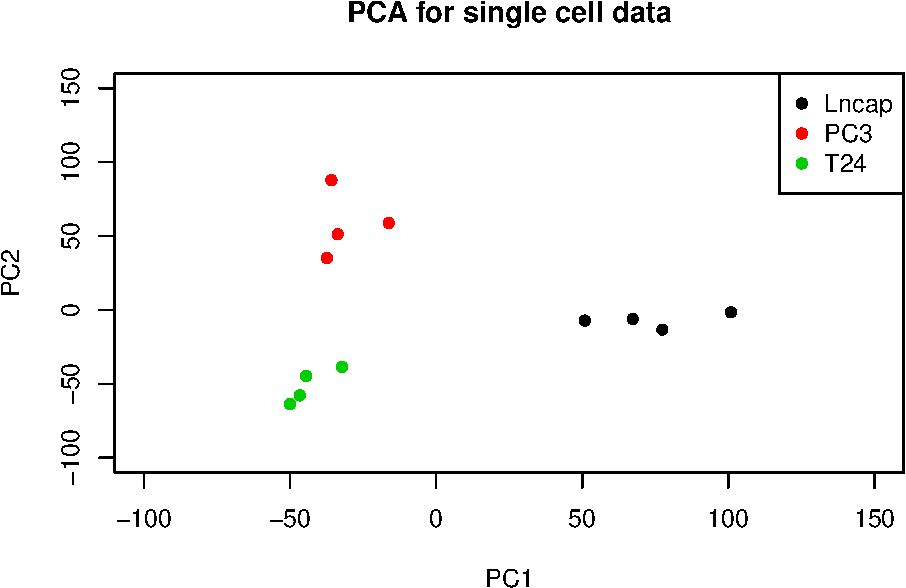
\includegraphics{Project_jankauskaite_ugne_files/figure-latex/unnamed-chunk-11-1.pdf}

\paragraph{One-way ANOVA Test}\label{one-way-anova-test}

A shift of one (to avoid log(0)) is applied and log2 of RPKM counts
taken for easier calculation and imaging.

\begin{Shaded}
\begin{Highlighting}[]
\NormalTok{data.RPKM_12cancer[,}\DecValTok{2}\OperatorTok{:}\DecValTok{13}\NormalTok{] <-}\StringTok{ }\KeywordTok{log2}\NormalTok{(data.RPKM_12cancer[,}\DecValTok{2}\OperatorTok{:}\DecValTok{13}\NormalTok{]}\OperatorTok{+}\DecValTok{1}\NormalTok{)}
\end{Highlighting}
\end{Shaded}

Then we can perform one-way ANOVA test with Benjamin-Hochberg p-value
adjustment and post-hoc Tukey test.

\begin{enumerate}
\def\labelenumi{\arabic{enumi}.}
\tightlist
\item
  Create some helper variables
\end{enumerate}

\begin{Shaded}
\begin{Highlighting}[]
\CommentTok{# threshold p-value}
\NormalTok{p_t=}\FloatTok{0.05}
\CommentTok{# some helper data frames for data separation and storage}
\NormalTok{PC3vsLncap =}\StringTok{ }\KeywordTok{data.frame}\NormalTok{(}\DataTypeTok{Gene=}\KeywordTok{character}\NormalTok{(),  }\DataTypeTok{p.Tukey=}\KeywordTok{double}\NormalTok{(), }\DataTypeTok{stringsAsFactors=}\OtherTok{FALSE}\NormalTok{)}
\NormalTok{T24vsLncap =}\StringTok{ }\KeywordTok{data.frame}\NormalTok{(}\DataTypeTok{Gene=}\KeywordTok{character}\NormalTok{(),  }\DataTypeTok{p.Tukey=}\KeywordTok{double}\NormalTok{(), }\DataTypeTok{stringsAsFactors=}\OtherTok{FALSE}\NormalTok{)}
\NormalTok{T24vsPC3 =}\StringTok{ }\KeywordTok{data.frame}\NormalTok{(}\DataTypeTok{Gene=}\KeywordTok{character}\NormalTok{(),  }\DataTypeTok{p.Tukey=}\KeywordTok{double}\NormalTok{(), }\DataTypeTok{stringsAsFactors=}\OtherTok{FALSE}\NormalTok{)}
\NormalTok{ANOVA=}\KeywordTok{data.frame}\NormalTok{(}\DataTypeTok{Gene=}\KeywordTok{character}\NormalTok{(), }\DataTypeTok{p=}\KeywordTok{double}\NormalTok{(), }\DataTypeTok{q=}\KeywordTok{double}\NormalTok{())}
\end{Highlighting}
\end{Shaded}

\begin{enumerate}
\def\labelenumi{\arabic{enumi}.}
\setcounter{enumi}{1}
\tightlist
\item
  Run one-way ANOVA and Tukey post-hoc
\end{enumerate}

\begin{Shaded}
\begin{Highlighting}[]
\NormalTok{tmydf =}\StringTok{ }\KeywordTok{setNames}\NormalTok{(}\KeywordTok{data.frame}\NormalTok{(}\KeywordTok{t}\NormalTok{(data.RPKM_12cancer[,}\OperatorTok{-}\DecValTok{1}\NormalTok{])), data.RPKM_12cancer[,}\DecValTok{1}\NormalTok{])}
\NormalTok{s<-}\KeywordTok{data.frame}\NormalTok{(}\DataTypeTok{CellType=}\KeywordTok{factor}\NormalTok{(}\KeywordTok{c}\NormalTok{(}\KeywordTok{rep}\NormalTok{(}\StringTok{"Lncap"}\NormalTok{, Lncap.num_files),}
                     \KeywordTok{rep}\NormalTok{(}\StringTok{"PC3"}\NormalTok{, PC3.num_files), }\KeywordTok{rep}\NormalTok{(}\StringTok{"T24"}\NormalTok{, T24.num_files))), tmydf)}
\NormalTok{num_genes =}\StringTok{ }\KeywordTok{dim}\NormalTok{(s)[}\DecValTok{2}\NormalTok{]}
\ControlFlowTok{for}\NormalTok{ (i }\ControlFlowTok{in} \DecValTok{2}\OperatorTok{:}\NormalTok{num_genes)\{}
\NormalTok{  geneCounts <-}\StringTok{ }\NormalTok{s[,i]}
\NormalTok{  geneName <-}\StringTok{ }\KeywordTok{names}\NormalTok{(s[i])}
\NormalTok{  model<-}\KeywordTok{lm}\NormalTok{(geneCounts}\OperatorTok{~}\NormalTok{s}\OperatorTok{$}\NormalTok{CellType)}
\NormalTok{  an <-}\StringTok{ }\KeywordTok{anova}\NormalTok{(model)}
\NormalTok{  an.p <-}\StringTok{ }\NormalTok{an}\OperatorTok{$}\StringTok{`}\DataTypeTok{Pr(>F)}\StringTok{`}\NormalTok{[}\DecValTok{1}\NormalTok{]}
\NormalTok{  ANOVA =}\StringTok{ }\KeywordTok{rbind}\NormalTok{(ANOVA, }\KeywordTok{data.frame}\NormalTok{(}\DataTypeTok{Gene=}\NormalTok{geneName, }\DataTypeTok{p=}\NormalTok{an.p))}

\NormalTok{  posthoc <-}\StringTok{ }\KeywordTok{TukeyHSD}\NormalTok{(}\KeywordTok{aov}\NormalTok{(geneCounts}\OperatorTok{~}\NormalTok{s}\OperatorTok{$}\NormalTok{CellType))}
  \ControlFlowTok{for}\NormalTok{ (j }\ControlFlowTok{in} \DecValTok{1}\OperatorTok{:}\DecValTok{3}\NormalTok{) \{}
\NormalTok{    tukey.p <-}\StringTok{ }\NormalTok{posthoc}\OperatorTok{$}\StringTok{`}\DataTypeTok{s$CellType}\StringTok{`}\NormalTok{[j,}\DecValTok{4}\NormalTok{]}
\NormalTok{    rowName =}\StringTok{ }\KeywordTok{rownames}\NormalTok{(posthoc}\OperatorTok{$}\StringTok{`}\DataTypeTok{s$CellType}\StringTok{`}\NormalTok{)[j]}
    \ControlFlowTok{if}\NormalTok{ (}\KeywordTok{identical}\NormalTok{(rowName,}\StringTok{"PC3-Lncap"}\NormalTok{))\{}
\NormalTok{      PC3vsLncap =}\StringTok{ }\KeywordTok{rbind}\NormalTok{(PC3vsLncap, }\KeywordTok{data.frame}\NormalTok{(}\DataTypeTok{Gene=}\NormalTok{geneName, }\DataTypeTok{p.Tukey=}\NormalTok{tukey.p))}
\NormalTok{    \}}
    \ControlFlowTok{else} \ControlFlowTok{if}\NormalTok{ (}\KeywordTok{identical}\NormalTok{(rowName,}\StringTok{"T24-Lncap"}\NormalTok{))\{}
\NormalTok{       T24vsLncap =}\StringTok{ }\KeywordTok{rbind}\NormalTok{(T24vsLncap, }\KeywordTok{data.frame}\NormalTok{(}\DataTypeTok{Gene=}\NormalTok{geneName, }\DataTypeTok{p.Tukey=}\NormalTok{tukey.p))}
\NormalTok{    \}}
    \ControlFlowTok{else} \ControlFlowTok{if}\NormalTok{ (}\KeywordTok{identical}\NormalTok{(rowName,}\StringTok{"T24-PC3"}\NormalTok{))\{}
\NormalTok{       T24vsPC3 =}\StringTok{ }\KeywordTok{rbind}\NormalTok{(T24vsPC3, }\KeywordTok{data.frame}\NormalTok{(}\DataTypeTok{Gene=}\NormalTok{geneName, }\DataTypeTok{p.Tukey=}\NormalTok{tukey.p))}
\NormalTok{    \}}
\NormalTok{  \}}
\NormalTok{\}}
\end{Highlighting}
\end{Shaded}

Number of genes with unadjusted ANOVA p-values less than 0.05:

\begin{verbatim}
## [1] 3191
\end{verbatim}

\begin{enumerate}
\def\labelenumi{\arabic{enumi}.}
\setcounter{enumi}{2}
\tightlist
\item
  Benjamin-Hochberg ANOVA p-value adjustment
\end{enumerate}

\begin{Shaded}
\begin{Highlighting}[]
\CommentTok{#Use BH to adjust p values}
\NormalTok{ANOVA}\OperatorTok{$}\NormalTok{q <-}\StringTok{ }\KeywordTok{p.adjust}\NormalTok{(ANOVA}\OperatorTok{$}\NormalTok{p, }\DataTypeTok{method =} \StringTok{"BH"}\NormalTok{)}
\end{Highlighting}
\end{Shaded}

Number of genes with BH adjusted ANOVA p-value (q) less than 0.05:

\begin{verbatim}
## [1] 928
\end{verbatim}

Add newly calculated p values to the dataframe:

\begin{Shaded}
\begin{Highlighting}[]
\NormalTok{data.RPKM_12cancer}\OperatorTok{$}\NormalTok{p.ANOVA <-}\StringTok{ }\NormalTok{ANOVA}\OperatorTok{$}\NormalTok{p}
\NormalTok{data.RPKM_12cancer}\OperatorTok{$}\NormalTok{q.ANOVA <-}\StringTok{ }\NormalTok{ANOVA}\OperatorTok{$}\NormalTok{q}
\NormalTok{data.RPKM_12cancer}\OperatorTok{$}\NormalTok{PC3vsLncap.p.Tukey <-}\StringTok{ }\NormalTok{PC3vsLncap}\OperatorTok{$}\NormalTok{p.Tukey}
\NormalTok{data.RPKM_12cancer}\OperatorTok{$}\NormalTok{T24vsLncap.p.Tukey <-}\StringTok{ }\NormalTok{T24vsLncap}\OperatorTok{$}\NormalTok{p.Tukey}
\NormalTok{data.RPKM_12cancer}\OperatorTok{$}\NormalTok{T24vsPC3.p.Tukey <-}\StringTok{ }\NormalTok{T24vsPC3}\OperatorTok{$}\NormalTok{p.Tukey}
\end{Highlighting}
\end{Shaded}

Genes are considered differentially expressed between two types of cells
if both BH adjusted ANOVA p-value (q) and Tukey p value are smaller than
0.05.

\begin{Shaded}
\begin{Highlighting}[]
\NormalTok{id.de_PC3vsLncap <-}\StringTok{ }\KeywordTok{which}\NormalTok{(data.RPKM_12cancer}\OperatorTok{$}\NormalTok{q.ANOVA }\OperatorTok{<}\StringTok{ }\NormalTok{p_t }\OperatorTok{&}
\StringTok{                            }\NormalTok{data.RPKM_12cancer}\OperatorTok{$}\NormalTok{PC3vsLncap.p.Tukey }\OperatorTok{<}\StringTok{ }\NormalTok{p_t)}
\NormalTok{id.de_T24vsLncap <-}\StringTok{ }\KeywordTok{which}\NormalTok{(data.RPKM_12cancer}\OperatorTok{$}\NormalTok{q.ANOVA }\OperatorTok{<}\StringTok{ }\NormalTok{p_t }\OperatorTok{&}
\StringTok{                            }\NormalTok{data.RPKM_12cancer}\OperatorTok{$}\NormalTok{T24vsLncap.p.Tukey }\OperatorTok{<}\StringTok{ }\NormalTok{p_t)}
\NormalTok{id.de_T24vsPC3 <-}\StringTok{ }\KeywordTok{which}\NormalTok{(data.RPKM_12cancer}\OperatorTok{$}\NormalTok{q.ANOVA }\OperatorTok{<}\StringTok{ }\NormalTok{p_t }\OperatorTok{&}
\StringTok{                          }\NormalTok{data.RPKM_12cancer}\OperatorTok{$}\NormalTok{T24vsPC3.p.Tukey }\OperatorTok{<}\StringTok{ }\NormalTok{p_t)}
\end{Highlighting}
\end{Shaded}

Number of DE genes between PC3 and Lncap cells:

\begin{verbatim}
## [1] 676
\end{verbatim}

Number of DE genes between T24 and Lncap cells:

\begin{verbatim}
## [1] 784
\end{verbatim}

Number of DE genes between T24 and PC3 cells:

\begin{verbatim}
## [1] 476
\end{verbatim}

The number of pairwise differentially expressed genes are higher than in
the original publication. However, proportional relationship is
maintained.

\subsubsection{Differenial Expression Analysis of Circulating Tumor
Transcriptomes}\label{differenial-expression-analysis-of-circulating-tumor-transcriptomes}

Circulating tumor samples samples are separated from the rest data.
Shift of 1 and log2 is applied to RPKM counts.

\begin{Shaded}
\begin{Highlighting}[]
\NormalTok{data.RPKM_tumor<-}\KeywordTok{data.frame}\NormalTok{(}\DataTypeTok{Genes=}\NormalTok{data.RPKM}\OperatorTok{$}\NormalTok{Gene, }\KeywordTok{log2}\NormalTok{(data.RPKM[,}\DecValTok{2}\OperatorTok{:}\DecValTok{16}\NormalTok{]}\OperatorTok{+}\DecValTok{1}\NormalTok{))}
\KeywordTok{dim}\NormalTok{(data.RPKM_tumor)}
\end{Highlighting}
\end{Shaded}

\begin{verbatim}
## [1] 24607    16
\end{verbatim}

\paragraph{One-way ANOVA Test}\label{one-way-anova-test-1}

Then we can perform one-way ANOVA test with Benjamin-Hochberg p-value
adjustment and post-hoc Tukey test. Since calculations are equivalent to
the ones for 12 single cell data, they are excluded from PDF report
file. To see the code please refer to the R markdown file.

The number of genes for which ANOVA p-values are less then 0.05 is:

\begin{verbatim}
## [1] 2266
\end{verbatim}

Number of genes with BH adjusted ANOVA p-value (q) less than 0.05:

\begin{verbatim}
## [1] 567
\end{verbatim}

Now, we can obtain number of genes that are differentially expressed
between primary melanocytes and circulating tumor cells:

\begin{Shaded}
\begin{Highlighting}[]
\NormalTok{id.de_PMvsCTC <-}\StringTok{ }\KeywordTok{which}\NormalTok{(data.RPKM_tumor}\OperatorTok{$}\NormalTok{q.ANOVA }\OperatorTok{<}\StringTok{ }\NormalTok{p_t }\OperatorTok{&}
\StringTok{                         }\NormalTok{data.RPKM_tumor}\OperatorTok{$}\NormalTok{PMvsCTC.p.Tukey }\OperatorTok{<}\StringTok{ }\NormalTok{p_t)}
\KeywordTok{length}\NormalTok{(id.de_PMvsCTC)}
\end{Highlighting}
\end{Shaded}

\begin{verbatim}
## [1] 302
\end{verbatim}

Number of genes that are upregulated in putative CTCs in comparison to
primary melanocytes and first rows of these genes expression data:

\begin{verbatim}
## [1] 138
\end{verbatim}

\begin{table}[H]
\centering\rowcolors{2}{gray!6}{white}

\resizebox{\linewidth}{!}{\begin{tabular}{lrrrrrrrrrrr}
\hiderowcolors
\toprule
  & CTC1 & CTC2 & CTC3 & CTC4 & CTC5 & CTC6 & PM1 & PM2 & p.ANOVA & q.ANOVA & PMvsCTC.p.Tukey\\
\midrule
\showrowcolors
NIPAL3+STPG1 & 3.862232 & 6.873917 & 6.504492 & 6.164927 & 3.981111 & 4.713672 & 0.1239859 & 0.0697603 & 0.0014223 & 0.0392243 & 0.0009325\\
CDC20 & 5.471837 & 4.761157 & 5.642079 & 3.707087 & 3.982662 & 4.651315 & 0.0000000 & 0.2893640 & 0.0000228 & 0.0021208 & 0.0002422\\
PSMB4 & 11.927822 & 11.511092 & 11.207168 & 10.936159 & 11.254160 & 10.694366 & 9.4784719 & 9.7895465 & 0.0000207 & 0.0019719 & 0.0054582\\
IQGAP3 & 7.313902 & 3.662955 & 6.707367 & 5.291382 & 1.694006 & 7.030844 & 0.0932843 & 0.0000000 & 0.0012797 & 0.0365825 & 0.0088873\\
SERTAD4 & 5.125461 & 2.997635 & 6.123106 & 3.783732 & 2.033973 & 3.134272 & 0.0000000 & 0.0000000 & 0.0006068 & 0.0224578 & 0.0063098\\
ENAH & 6.039267 & 3.248495 & 5.155749 & 5.767513 & 3.710193 & 5.717252 & 0.0758166 & 0.0535427 & 0.0014445 & 0.0396036 & 0.0014777\\
\bottomrule
\end{tabular}}
\rowcolors{2}{white}{white}
\end{table}

Number of genes that are downregulated in putative CTCs in comparison to
primary melanocytes and first rows of these genes expression data:

\begin{verbatim}
## [1] 164
\end{verbatim}

\begin{table}[H]
\centering\rowcolors{2}{gray!6}{white}

\resizebox{\linewidth}{!}{\begin{tabular}{lrrrrrrrrrrr}
\hiderowcolors
\toprule
  & CTC1 & CTC2 & CTC3 & CTC4 & CTC5 & CTC6 & PM1 & PM2 & p.ANOVA & q.ANOVA & PMvsCTC.p.Tukey\\
\midrule
\showrowcolors
ISG15 & 0.000000 & 0.0000000 & 0.0000000 & 3.714270 & 0.000000 & 0.000000 & 9.3696997 & 8.1844807 & 0.0000107 & 0.0011227 & 0.0000134\\
MFAP2 & 0.000000 & 0.3918379 & 0.0000000 & 0.000000 & 0.000000 & 0.000000 & 5.4878813 & 4.8870950 & 0.0000000 & 0.0000000 & 0.0000000\\
NBPF3 & 0.000000 & 0.1870653 & 0.0000000 & 0.000000 & 0.000000 & 0.000000 & 0.6582337 & 0.3197848 & 0.0002087 & 0.0105568 & 0.0002798\\
RUNX3 & 3.321721 & 0.0000000 & 0.0406248 & 2.978488 & 0.000000 & 0.000000 & 5.2672186 & 5.5126099 & 0.0004947 & 0.0194142 & 0.0058986\\
TRIM63 & 0.000000 & 0.0000000 & 0.0000000 & 0.000000 & 0.000000 & 0.000000 & 2.8865314 & 6.5809734 & 0.0010607 & 0.0323831 & 0.0087888\\
IFI6 & 6.793634 & 5.5332812 & 5.5186124 & 6.405115 & 6.638209 & 4.455067 & 10.8136311 & 10.9901242 & 0.0000672 & 0.0046739 & 0.0000672\\
\bottomrule
\end{tabular}}
\rowcolors{2}{white}{white}
\end{table}

\paragraph{Hierarchial Clustering}\label{hierarchial-clustering}

As in the original paper, hierarchical clustering was performed only for
genes for which at least one sample had a high expression value (RPKM
\textgreater{} 100).

\begin{Shaded}
\begin{Highlighting}[]
\CommentTok{# Rearange data}
\NormalTok{row_names <-}\StringTok{ }\NormalTok{data.RPKM[,}\DecValTok{1}\NormalTok{]}
\NormalTok{data.RPKM <-}\StringTok{ }\NormalTok{data.RPKM[,}\OperatorTok{-}\DecValTok{1}\NormalTok{]}
\KeywordTok{rownames}\NormalTok{(data.RPKM) <-}\StringTok{ }\NormalTok{row_names}
\KeywordTok{print}\NormalTok{(}\KeywordTok{paste0}\NormalTok{(}\StringTok{"Original data gene count: "}\NormalTok{, }\KeywordTok{dim}\NormalTok{(data.RPKM)[}\DecValTok{1}\NormalTok{]))}
\end{Highlighting}
\end{Shaded}

\begin{verbatim}
## [1] "Original data gene count: 24607"
\end{verbatim}

\begin{Shaded}
\begin{Highlighting}[]
\CommentTok{# get highly expressed genes}
\NormalTok{data.RPKM_high <-}\StringTok{ }\NormalTok{data.RPKM[}\KeywordTok{apply}\NormalTok{(data.RPKM[,}\OperatorTok{-}\DecValTok{1}\NormalTok{], }\DecValTok{1}\NormalTok{, }\ControlFlowTok{function}\NormalTok{(row) \{}\KeywordTok{any}\NormalTok{(row }\OperatorTok{>}\StringTok{ }\DecValTok{100}\NormalTok{)\}), ]}
\KeywordTok{colnames}\NormalTok{(data.RPKM_high) <-}\StringTok{ }\NormalTok{group}
\KeywordTok{print}\NormalTok{(}\KeywordTok{paste0}\NormalTok{(}\StringTok{"Gene count for genes with RPKM > 100: "}\NormalTok{, }\KeywordTok{dim}\NormalTok{(data.RPKM_high)[}\DecValTok{1}\NormalTok{]))}
\end{Highlighting}
\end{Shaded}

\begin{verbatim}
## [1] "Gene count for genes with RPKM > 100: 4587"
\end{verbatim}

To cluster data, dissimilarity distance is calculated based on Spearman
correlation and 1000 bootstrapped samples added.

\begin{Shaded}
\begin{Highlighting}[]
\NormalTok{spearman <-}\StringTok{ }\ControlFlowTok{function}\NormalTok{(x, ...) \{}
\NormalTok{    x <-}\StringTok{ }\KeywordTok{as.matrix}\NormalTok{(x)}
\NormalTok{    res <-}\StringTok{ }\KeywordTok{as.dist}\NormalTok{(}\DecValTok{1} \OperatorTok{-}\StringTok{ }\KeywordTok{cor}\NormalTok{(x, }\DataTypeTok{method =} \StringTok{"spearman"}\NormalTok{, }\DataTypeTok{use =} \StringTok{"everything"}\NormalTok{))}
\NormalTok{    res <-}\StringTok{ }\KeywordTok{as.dist}\NormalTok{(res)}
    \KeywordTok{attr}\NormalTok{(res, }\StringTok{"method"}\NormalTok{) <-}\StringTok{ "spearman"}
    \KeywordTok{return}\NormalTok{(res)}
\NormalTok{\}}
\NormalTok{data.RPKM_high <-}\StringTok{ }\NormalTok{data.RPKM_high[, }\OperatorTok{!}\StringTok{ }\KeywordTok{apply}\NormalTok{(data.RPKM_high , }\DecValTok{2}\NormalTok{ ,}
                                           \ControlFlowTok{function}\NormalTok{(x) }\KeywordTok{sd}\NormalTok{(x, }\DataTypeTok{na.rm =} \OtherTok{TRUE}\NormalTok{)}\OperatorTok{==}\DecValTok{0}\NormalTok{ ) ]}
\NormalTok{cluster.bootstrap <-}\StringTok{ }\KeywordTok{pvclust}\NormalTok{(data.RPKM_high, }\DataTypeTok{parallel =} \OtherTok{TRUE}\NormalTok{, }\DataTypeTok{nboot =} \DecValTok{1000}\NormalTok{,}
                             \DataTypeTok{method.dist=}\NormalTok{spearman)}
\end{Highlighting}
\end{Shaded}

\begin{verbatim}
## Creating a temporary cluster...done:
## socket cluster with 7 nodes on host 'localhost'
## Multiscale bootstrap... Done.
\end{verbatim}

In the plot below, \textcolor{red}{AU} (Approximately Unbiased) p-value
and \textcolor{green}{BP} (Bootstrap Probability) value are as described
in the Methods section. Red rectangles marks clusters with high AU
values (95\%).

\begin{Shaded}
\begin{Highlighting}[]
\NormalTok{dend <-}\StringTok{ }\KeywordTok{as.dendrogram}\NormalTok{(cluster.bootstrap)}
\NormalTok{dend <-}\StringTok{ }\KeywordTok{color_branches}\NormalTok{(dend, }\DecValTok{4}\NormalTok{)}

\NormalTok{dend }\OperatorTok\StringTok{ }\NormalTok{as.dendrogram }\OperatorTok
\StringTok{   }\KeywordTok{plot}\NormalTok{(}\DataTypeTok{main =} \StringTok{"Cluster dendrogram with AU/BP values (%)}\CharTok{\textbackslash{}n}
\StringTok{        reproduced plot with dendrogram"}\NormalTok{,}
        \DataTypeTok{ylab =} \StringTok{"1 - Spearman correlation"}\NormalTok{)}
\NormalTok{cluster.bootstrap }\OperatorTok\StringTok{ }\KeywordTok{text}\NormalTok{(}\DataTypeTok{cex=}\FloatTok{0.6}\NormalTok{)}
\NormalTok{cluster.bootstrap }\OperatorTok\StringTok{ }\KeywordTok{pvrect}\NormalTok{(}\DataTypeTok{alpha=}\FloatTok{0.95}\NormalTok{, }\DataTypeTok{pv=}\StringTok{"au"}\NormalTok{, }\DataTypeTok{type=}\StringTok{"geq"}\NormalTok{)}
\end{Highlighting}
\end{Shaded}

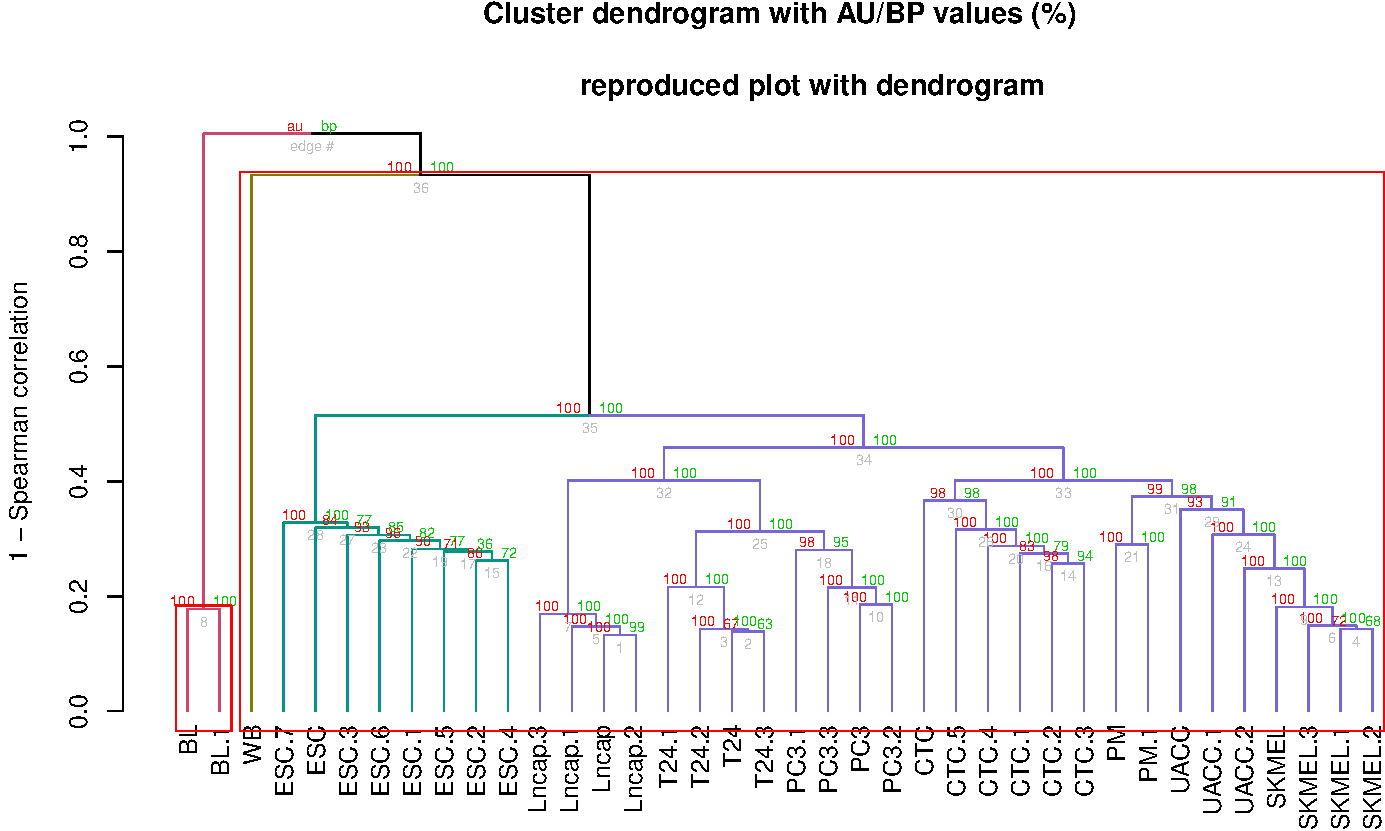
\includegraphics{Project_jankauskaite_ugne_files/figure-latex/unnamed-chunk-34-1.pdf}

Overall, all cells clustered within their cell lines with high AU
p-value. Burkitt's lymphoma samples are clearly separated from prostate
and bladder single cell samples, primary melanocytes, melanoma cancer
cell line and embryonic stem cell samples. All the rest samples make
expected clusters with samples of similar cell lines, importantly CTC
are in the same cluster as PM, SKMEL and UACC cells.

\subparagraph{Heatmap Comparison of Gene
Expression}\label{heatmap-comparison-of-gene-expression}

For the heatmaps, the data shift value before taking a logarithm of the
data was not stated in the original paper. However, since heatmaps in
\textbf{figures 4b-4f} of the paper include negative logarithm values,
here the applied shift is chosen so be smaller then one:

\begin{Shaded}
\begin{Highlighting}[]
\NormalTok{data.RPKM_log <-}\StringTok{ }\KeywordTok{log2}\NormalTok{(data.RPKM}\OperatorTok{+}\FloatTok{0.1}\NormalTok{)}
\end{Highlighting}
\end{Shaded}

In \textbf{figure 4b} and \textbf{supplementary figure 9} Ramskold
\emph{et al.} used known NG2+ CTC marker genes PMEL, MITF, TYR, MLANA
and known immune marker genes PTPRC, CD53, CCL5 to show that CTCs are of
melanocytic origin and not immune origin. These results are accurately
reproduced in the figure below:

\begin{Shaded}
\begin{Highlighting}[]
\NormalTok{cols <-}\StringTok{ }\KeywordTok{c}\NormalTok{(}\DecValTok{1}\OperatorTok{:}\DecValTok{23}\NormalTok{, }\DecValTok{36}\OperatorTok{:}\DecValTok{39}\NormalTok{)}
\NormalTok{data.RPKM_h1 <-}\StringTok{ }\KeywordTok{rbind}\NormalTok{(data.RPKM_log[}\StringTok{"PMEL"}\NormalTok{, cols], data.RPKM_log[}\StringTok{"MITF"}\NormalTok{, cols],}
\NormalTok{                      data.RPKM_log[}\StringTok{"TYR"}\NormalTok{, cols], data.RPKM_log[}\StringTok{"MLANA"}\NormalTok{, cols],}
\NormalTok{                      data.RPKM_log[}\StringTok{"PTPRC"}\NormalTok{, cols], data.RPKM_log[}\StringTok{"CD53"}\NormalTok{, cols],}
\NormalTok{                      data.RPKM_log[}\StringTok{"CCL5"}\NormalTok{, cols])}
\KeywordTok{colnames}\NormalTok{(data.RPKM_h1) <-}\StringTok{ }\NormalTok{group[cols]}

\KeywordTok{heatmap.2}\NormalTok{(}\KeywordTok{as.matrix}\NormalTok{(data.RPKM_h1), }\DataTypeTok{dendrogram =} \StringTok{"none"}\NormalTok{, }\DataTypeTok{Colv=}\OtherTok{FALSE}\NormalTok{, }\DataTypeTok{Rowv =} \OtherTok{FALSE}\NormalTok{,}
          \DataTypeTok{tracecol =} \OtherTok{NA}\NormalTok{, }\DataTypeTok{col=}\KeywordTok{colorRampPalette}\NormalTok{(}\KeywordTok{c}\NormalTok{(}\StringTok{"white"}\NormalTok{, }\StringTok{"red"}\NormalTok{)),}
          \DataTypeTok{breaks=}\KeywordTok{c}\NormalTok{(}\DecValTok{1}\OperatorTok{:}\FloatTok{0.5}\OperatorTok{:}\DecValTok{10}\NormalTok{), }\DataTypeTok{density.info=}\StringTok{"none"}\NormalTok{, }\DataTypeTok{key.xlab =} \StringTok{"RPKM log2"}\NormalTok{, }\DataTypeTok{cexRow =} \DecValTok{1}\NormalTok{)}
\end{Highlighting}
\end{Shaded}

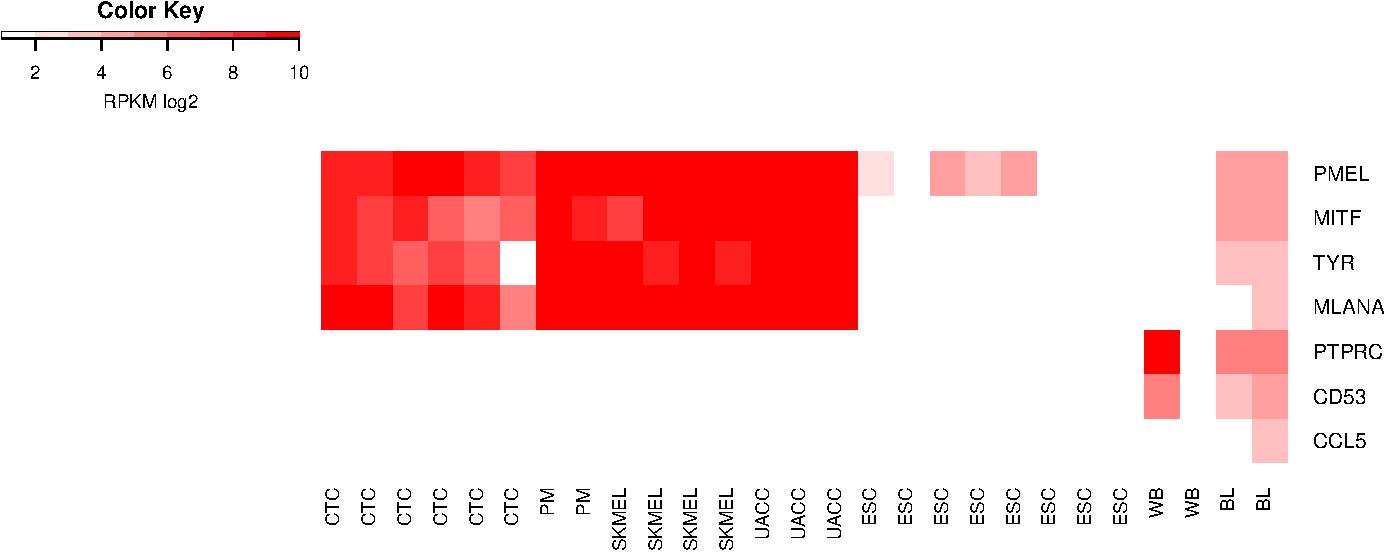
\includegraphics{Project_jankauskaite_ugne_files/figure-latex/unnamed-chunk-36-1.pdf}

Then, in order to further compare primary melanocytes and CTCs, the
authors showed that melanoma-associated tumor antigens are upregulated
in CTC samples, compared to PM samples. These results were reproduced in
the figure below:

\begin{Shaded}
\begin{Highlighting}[]
\NormalTok{cols <-}\StringTok{ }\KeywordTok{c}\NormalTok{(}\DecValTok{1}\OperatorTok{:}\DecValTok{23}\NormalTok{, }\DecValTok{36}\OperatorTok{:}\DecValTok{39}\NormalTok{)}
\NormalTok{data.RPKM_h2 <-}\StringTok{ }\KeywordTok{rbind}\NormalTok{(data.RPKM_log[}\StringTok{"MAGEB2"}\NormalTok{, cols], data.RPKM_log[}\StringTok{"MAGEC2"}\NormalTok{, cols],}
\NormalTok{                      data.RPKM_log[}\StringTok{"MAGEA10"}\NormalTok{, cols], data.RPKM_log[}\StringTok{"MAGEA2"}\NormalTok{, cols],}
\NormalTok{                      data.RPKM_log[}\StringTok{"CSAG4+MAGEA12"}\NormalTok{, cols], data.RPKM_log[}\StringTok{"MAGEA6"}\NormalTok{, cols],}
\NormalTok{                      data.RPKM_log[}\StringTok{"MAGEA3"}\NormalTok{, cols])}
\KeywordTok{colnames}\NormalTok{(data.RPKM_h2) <-}\StringTok{ }\NormalTok{group[cols]}

\KeywordTok{heatmap.2}\NormalTok{(}\KeywordTok{as.matrix}\NormalTok{(data.RPKM_h2), }\DataTypeTok{dendrogram =} \StringTok{"none"}\NormalTok{, }\DataTypeTok{Colv=}\OtherTok{FALSE}\NormalTok{, }\DataTypeTok{Rowv =} \OtherTok{FALSE}\NormalTok{,}
          \DataTypeTok{tracecol =} \OtherTok{NA}\NormalTok{, }\DataTypeTok{col=}\KeywordTok{colorRampPalette}\NormalTok{(}\KeywordTok{c}\NormalTok{(}\StringTok{"blue"}\NormalTok{, }\StringTok{"white"}\NormalTok{, }\StringTok{"red"}\NormalTok{)),}
          \DataTypeTok{breaks=}\KeywordTok{c}\NormalTok{(}\OperatorTok{-}\DecValTok{5}\OperatorTok{:}\DecValTok{5}\NormalTok{), }\DataTypeTok{key=}\OtherTok{TRUE}\NormalTok{, }\DataTypeTok{symkey=}\OtherTok{FALSE}\NormalTok{, }\DataTypeTok{density.info=}\StringTok{"none"}\NormalTok{,}
          \DataTypeTok{key.xlab =} \StringTok{"RPKM log2"}\NormalTok{, }\DataTypeTok{cexRow =} \DecValTok{1}\NormalTok{,}\DataTypeTok{margins=}\KeywordTok{c}\NormalTok{(}\DecValTok{5}\NormalTok{,}\DecValTok{18}\NormalTok{))}
\end{Highlighting}
\end{Shaded}

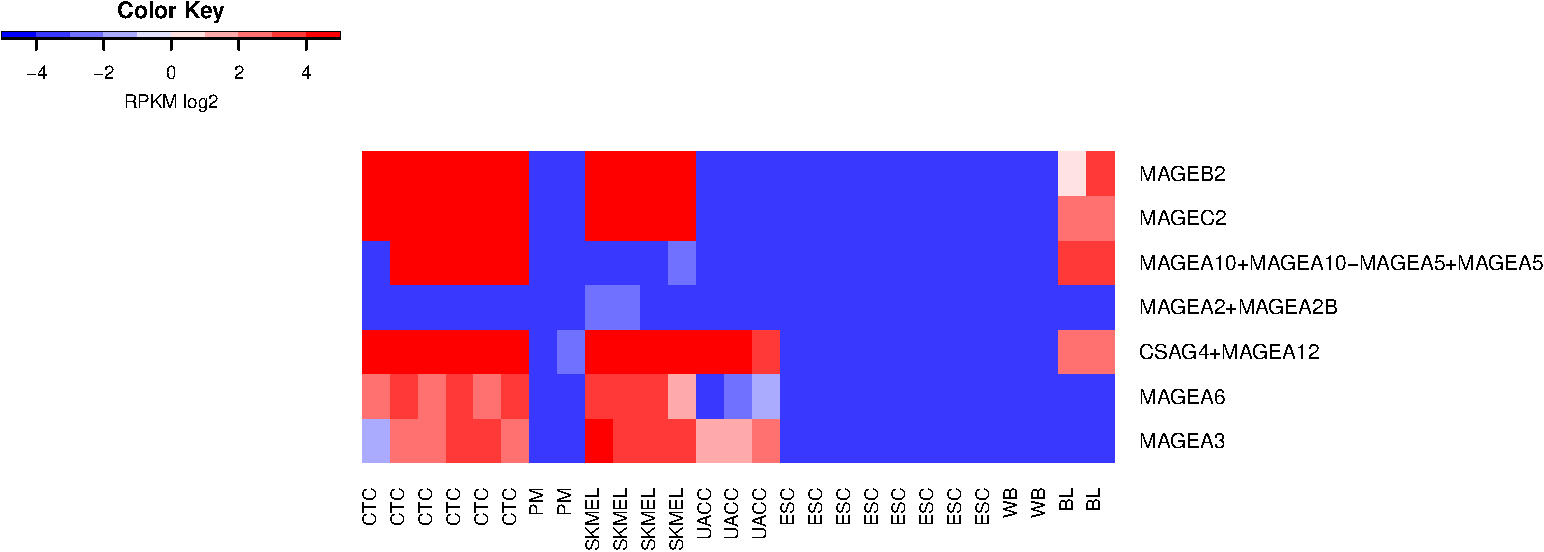
\includegraphics{Project_jankauskaite_ugne_files/figure-latex/unnamed-chunk-37-1.pdf}

Data table of these genes expression for CTC and PM samples shows clear
differential expression with significant one-way ANOVA p-values, BH
adjusted q-values, and Tukey post-hoc test p-values for all antigens,
except MAGEA2+MAGEA2B:

\begin{table}[H]
\centering\rowcolors{2}{gray!6}{white}

\resizebox{\linewidth}{!}{\begin{tabular}{lrrrrrrrrrrr}
\hiderowcolors
\toprule
  & CTC1 & CTC2 & CTC3 & CTC4 & CTC5 & CTC6 & PM1 & PM2 & p.ANOVA & q.ANOVA & PMvsCTC.p.Tukey\\
\midrule
\showrowcolors
MAGEB2 & 7.2237602 & 10.033935 & 7.598047 & 8.412136 & 9.092403 & 8.318488 & 0 & 0.0000000 & 0.0000000 & 0.0000095 & 0.0000004\\
MAGEC2 & 7.2164381 & 9.523607 & 9.352021 & 9.109006 & 8.911451 & 8.806244 & 0 & 0.0000000 & 0.0000000 & 0.0000022 & 0.0000001\\
MAGEA10+MAGEA10-MAGEA5+MAGEA5 & 0.0000000 & 7.909798 & 6.463821 & 6.299014 & 6.464823 & 5.917956 & 0 & 0.0000000 & 0.0016102 & 0.0422522 & 0.0187916\\
MAGEA2+MAGEA2B & 0.0000000 & 0.000000 & 0.000000 & 0.000000 & 0.000000 & 0.000000 & 0 & 0.0000000 & 0.1084233 & 0.4206824 & 1.0000000\\
CSAG4+MAGEA12 & 4.6219293 & 6.032660 & 6.858064 & 6.966196 & 6.478108 & 6.800355 & 0 & 0.1084925 & 0.0000487 & 0.0036797 & 0.0000567\\
\addlinespace
MAGEA6 & 2.9859013 & 3.908490 & 3.075102 & 3.210015 & 3.090047 & 3.798007 & 0 & 0.0000000 & 0.0000031 & 0.0004065 & 0.0000551\\
MAGEA3 & 0.3481506 & 2.707171 & 2.453360 & 3.258807 & 3.858179 & 2.733718 & 0 & 0.0000000 & 0.0037247 & 0.0737867 & 0.0184342\\
\bottomrule
\end{tabular}}
\rowcolors{2}{white}{white}
\end{table}

Further nine plasma-membrane associated transcripts were identified in
CTC compared to PM in the \textbf{figure 4e} of the original paper.
However, here the authors results are not reproduce completely. The
heatmap below shows that two of the nine transcripts - RPS3 and PSMB1 -
were also highly expressed in PM cells.

\begin{Shaded}
\begin{Highlighting}[]
\NormalTok{cols <-}\StringTok{ }\KeywordTok{c}\NormalTok{(}\DecValTok{1}\OperatorTok{:}\DecValTok{23}\NormalTok{, }\DecValTok{36}\OperatorTok{:}\DecValTok{39}\NormalTok{)}
\NormalTok{data.RPKM_h3 <-}\StringTok{ }\KeywordTok{rbind}\NormalTok{(data.RPKM_log[}\StringTok{"GJB1"}\NormalTok{, cols], data.RPKM_log[}\StringTok{"LL22NC03-63E9.3+PRAME"}\NormalTok{, cols],}
\NormalTok{                      data.RPKM_log[}\StringTok{"ADGRG6"}\NormalTok{, cols], data.RPKM_log[}\StringTok{"CRIM1"}\NormalTok{, cols],}
\NormalTok{                      data.RPKM_log[}\StringTok{"ABCG5"}\NormalTok{, cols], data.RPKM_log[}\StringTok{"SLC20A1"}\NormalTok{, cols],}
\NormalTok{                      data.RPKM_log[}\StringTok{"ADAM17"}\NormalTok{, cols], data.RPKM_log[}\StringTok{"RPS3"}\NormalTok{, cols],}
\NormalTok{                      data.RPKM_log[}\StringTok{"PSMB1"}\NormalTok{, cols])}
\KeywordTok{colnames}\NormalTok{(data.RPKM_h3) <-}\StringTok{ }\NormalTok{group[cols]}

\KeywordTok{library}\NormalTok{(gplots)}
\KeywordTok{heatmap.2}\NormalTok{(}\KeywordTok{as.matrix}\NormalTok{(data.RPKM_h3), }\DataTypeTok{dendrogram =} \StringTok{"none"}\NormalTok{, }\DataTypeTok{Colv=}\OtherTok{FALSE}\NormalTok{, }\DataTypeTok{Rowv=}\OtherTok{FALSE}\NormalTok{,}
          \DataTypeTok{tracecol =} \OtherTok{NA}\NormalTok{, }\DataTypeTok{col=}\KeywordTok{colorRampPalette}\NormalTok{(}\KeywordTok{c}\NormalTok{(}\StringTok{"blue"}\NormalTok{, }\StringTok{"white"}\NormalTok{, }\StringTok{"red"}\NormalTok{)),}
          \DataTypeTok{breaks=}\KeywordTok{c}\NormalTok{(}\OperatorTok{-}\DecValTok{10}\OperatorTok{:}\DecValTok{10}\NormalTok{), }\DataTypeTok{key=}\OtherTok{TRUE}\NormalTok{, }\DataTypeTok{symkey=}\OtherTok{FALSE}\NormalTok{, }\DataTypeTok{density.info=}\StringTok{"none"}\NormalTok{,}
          \DataTypeTok{key.xlab =} \StringTok{"RPKM log2"}\NormalTok{, }\DataTypeTok{cexRow =} \DecValTok{1}\NormalTok{, }\DataTypeTok{margins=}\KeywordTok{c}\NormalTok{(}\DecValTok{5}\NormalTok{,}\DecValTok{18}\NormalTok{))}
\end{Highlighting}
\end{Shaded}

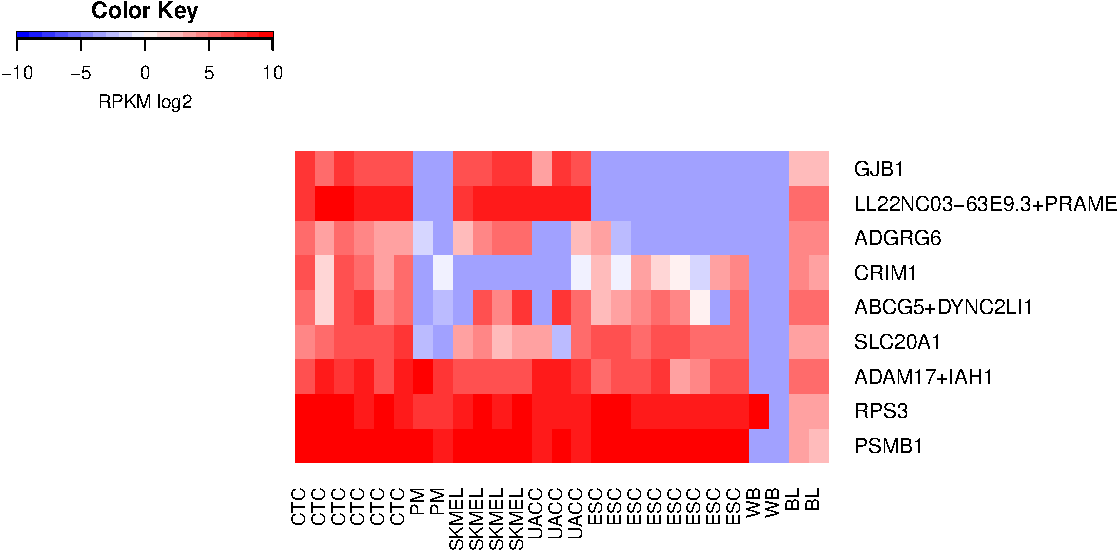
\includegraphics{Project_jankauskaite_ugne_files/figure-latex/unnamed-chunk-39-1.pdf}

Furthermore, comparing the authors data from Supplementary Table 4 to
data generated during this project, very similar results can be observed
for the nine genes (small differences may be due to different shift
before applying log2). It can be seen that genes RPS3 and PSMB1 are
quite highly expressed in PM according to the authors data, however in
the \textbf{figure 4e} of the paper the expression is shown as very
small.

\begin{itemize}
\tightlist
\item
  Data for 9 genes by Ramskold \emph{et al.}:
\end{itemize}

\begin{table}[H]
\centering\rowcolors{2}{gray!6}{white}

\resizebox{\linewidth}{!}{\begin{tabular}{llllllllllllllllllllllll}
\hiderowcolors
\toprule
  & ANOVA p-value & ANOVA q-value & skmel\_1 & skmel\_2 & skmel\_3 & skmel\_4 & uacc\_1 & uacc\_2 & uacc\_3 & pm\_1 & pm\_2 & ctc\_1 & ctc\_2 & ctc\_3 & ctc\_4 & ctc\_5 & ctc\_6 & pm-ctc & skmel-ctc & uacc-ctc & skmel-pm & uacc-pm & uacc-skmel\\
\midrule
\showrowcolors
GJB1 & 0.0000970759 & 0.0049404852 & 6.12 & 6.11 & 6.57 & 6.98 & 3.08 & 6.52 & 6.04 & 0.00 & 0.00 & 7.05 & 4.43 & 6.68 & 6.06 & 5.75 & 5.56 & 0.000110648 & 0.8606121831 & 0.7688454329 & 0.0000876726 & 0.0008702258 & 0.4380953055\\
PRAME & 0.0000000169 & 0.0000040282 & 7.18 & 7.82 & 7.91 & 7.72 & 7.62 & 8.09 & 8.18 & 0.00 & 0.00 & 6.90 & 9.14 & 8.63 & 7.95 & 8.34 & 7.61 & 0.0000000144 & 0.6515635278 & 0.9880147259 & 0.0000000454 & 0.000000052 & 0.8950328063\\
GPR126 & 0.0012470226 & 0.0304781205 & 2.37 & 3.53 & 5.38 & 4.39 & 0.00 & 0.00 & 2.24 & 0.00 & 0.00 & 4.51 & 3.07 & 4.73 & 4.05 & 3.11 & 2.41 & 0.0070193545 & 0.9782308143 & 0.0123044228 & 0.0064279949 & 0.86792823 & 0.0113745639\\
CRIM1 & 0.0007766786 & 0.0229789091 & 0.00 & 0.00 & 0.00 & 0.00 & 0.00 & 0.00 & 0.00 & 0.00 & 0.00 & 5.40 & 0.60 & 5.55 & 5.01 & 3.26 & 4.66 & 0.0109389433 & 0.0020642013 & 0.004074811 & 1 & 1 & 1\\
ABCG5 & 0.0011388686 & 0.0289473735 & 0.00 & 0.00 & 0.00 & 0.00 & 0.00 & 0.00 & 0.00 & 0.00 & 0.00 & 5.31 & 0.65 & 2.91 & 2.79 & 3.71 & 4.31 & 0.0147242625 & 0.0029404034 & 0.0056836826 & 1 & 1 & 1\\
\addlinespace
SLC20A1 & 0.0015717156 & 0.0359951974 & 2.62 & 3.66 & 1.64 & 2.62 & 3.18 & 0.00 & 5.16 & 0.00 & 0.00 & 4.19 & 4.91 & 6.33 & 5.84 & 5.78 & 6.79 & 0.0016237513 & 0.0240812314 & 0.0511150898 & 0.1688317914 & 0.1686737375 & 0.9989822561\\
ADAM17 & 0.0011468641 & 0.0289473735 & 4.25 & 2.81 & 3.44 & 3.03 & 6.62 & 2.58 & 4.29 & 0.00 & 0.00 & 5.71 & 3.48 & 5.77 & 6.35 & 5.02 & 5.24 & 0.0007327487 & 0.1065602584 & 0.780758385 & 0.0249646941 & 0.0057130703 & 0.5954955901\\
RPS3 & 0.0010898185 & 0.0283146755 & 12.18 & 12.70 & 12.59 & 12.75 & 11.85 & 12.19 & 11.82 & 11.23 & 11.03 & 12.68 & 13.35 & 13.14 & 12.43 & 13.38 & 12.12 & 0.0010110338 & 0.6519568294 & 0.0325484915 & 0.0064724161 & 0.1512022487 & 0.2355870606\\
PSMB1 & 0.0018572522 & 0.0398377849 & 10.01 & 9.69 & 9.80 & 10.08 & 8.48 & 9.32 & 8.06 & 9.86 & 8.45 & 10.13 & 9.86 & 10.33 & 10.51 & 10.85 & 10.37 & 0.0452155972 & 0.4934507157 & 0.0016155834 & 0.3196802873 & 0.6286366605 & 0.0217423522\\
\bottomrule
\end{tabular}}
\rowcolors{2}{white}{white}
\end{table}

\begin{itemize}
\tightlist
\item
  Data for 9 genes generated during this project:
\end{itemize}

\begin{table}[H]
\centering\rowcolors{2}{gray!6}{white}

\resizebox{\linewidth}{!}{\begin{tabular}{lrrrrrrrrrrrrrrrrrrrrrrr}
\hiderowcolors
\toprule
  & CTC1 & CTC2 & CTC3 & CTC4 & CTC5 & CTC6 & PM1 & PM2 & SKMEL1 & SKMEL2 & SKMEL3 & SKMEL4 & UACC1 & UACC2 & UACC3 & p.ANOVA & q.ANOVA & PMvsCTC.p.Tukey & SKMELvsCTC.p.Tukey & UACCvsCTC.p.Tukey & SKMELvsPM.p.Tukey & UACCvsPM.p.Tukey & UACCvsSKMEL.p.Tukey\\
\midrule
\showrowcolors
GJB1 & 7.824396 & 5.186566 & 7.381308 & 6.646872 & 6.454946 & 6.210213 & 0.0000000 & 0.0000000 & 6.774579 & 6.761906 & 7.219762 & 7.6432863 & 3.849982 & 7.2062825 & 6.6826237 & 0.0000312 & 0.0026269 & 0.0000337 & 0.8804247 & 0.7625852 & 0.0000302 & 0.0002590 & 0.4530095\\
LL22NC03-63E9.3+PRAME & 7.671798 & 9.907838 & 9.298326 & 8.538039 & 8.995661 & 8.034773 & 0.0000000 & 0.0000000 & 7.788570 & 8.483391 & 8.646811 & 8.3206468 & 8.334409 & 8.3367885 & 8.6932409 & 0.0000000 & 0.0000035 & 0.0000000 & 0.6860258 & 0.9032503 & 0.0000000 & 0.0000000 & 0.9882687\\
ADGRG6 & 5.161283 & 3.872159 & 5.167736 & 4.623820 & 3.887788 & 3.175038 & 0.4383693 & 0.0000000 & 3.131634 & 4.123306 & 5.933340 & 5.0954750 & 0.000000 & 0.0235495 & 3.0698949 & 0.0007718 & 0.0264125 & 0.0045787 & 0.9841691 & 0.0078299 & 0.0045197 & 0.8575949 & 0.0079317\\
CRIM1 & 6.036823 & 1.799073 & 6.232676 & 5.633584 & 4.031314 & 5.305246 & 0.0000000 & 0.6343014 & 0.000000 & 0.000000 & 0.000000 & 0.0172355 & 0.000000 & 0.0000000 & 0.9169042 & 0.0001073 & 0.0065024 & 0.0028044 & 0.0002391 & 0.0008918 & 0.9890369 & 0.9999995 & 0.9858419\\
ABCG5+DYNC2LI1 & 5.958574 & 2.231251 & 6.331449 & 7.526522 & 4.567064 & 5.356500 & 0.0000000 & 0.0638216 & 0.000000 & 6.647444 & 4.739803 & 7.2886904 & 0.000000 & 7.5157641 & 5.3263829 & 0.1708232 & 0.5149226 & 0.1298621 & 0.9801277 & 0.9436853 & 0.2456213 & 0.3509883 & 0.9974237\\
\addlinespace
SLC20A1 & 4.869780 & 5.497657 & 6.930370 & 6.337518 & 6.358833 & 7.386363 & 0.2011737 & 0.0000000 & 3.417988 & 4.330383 & 2.544618 & 3.4066786 & 4.020708 & 0.1373316 & 5.6608377 & 0.0014532 & 0.0396871 & 0.0011996 & 0.0447388 & 0.0542499 & 0.0809413 & 0.1224083 & 0.9989399\\
ADAM17+IAH1 & 6.330511 & 8.811522 & 7.895789 & 8.282476 & 6.022133 & 8.217339 & 9.0746712 & 7.5419164 & 6.535850 & 6.986341 & 6.977785 & 6.8434814 & 8.052411 & 8.6610982 & 7.2474001 & 0.2526594 & 0.6238995 & 0.7644026 & 0.5753344 & 0.9229178 & 0.2828689 & 0.9783528 & 0.3764294\\
RPS3 & 9.057396 & 9.728213 & 9.520673 & 8.744502 & 9.811728 & 8.425373 & 7.5235992 & 7.3320722 & 8.614279 & 9.081603 & 8.946302 & 9.1815132 & 8.648596 & 8.7324657 & 8.1259749 & 0.0022480 & 0.0537808 & 0.0015821 & 0.7846640 & 0.1427282 & 0.0076482 & 0.0754732 & 0.5287168\\
PSMB1 & 10.295304 & 10.120670 & 10.558845 & 10.702183 & 11.099917 & 10.539397 & 10.0833632 & 8.6621295 & 10.256641 & 9.944024 & 10.036955 & 10.3009553 & 8.944355 & 9.5981673 & 8.2963848 & 0.0030056 & 0.0640519 & 0.0492212 & 0.5511161 & 0.0028776 & 0.3075790 & 0.7656162 & 0.0334537\\
\bottomrule
\end{tabular}}
\rowcolors{2}{white}{white}
\end{table}

Finally, loss of expression in plasma-membrane proteins in CTCs was
investigated by the authors. The loss of membrane proteins makes cells
less visible for the immune system, thus can escape control, drift to
different regions of the body and cause metastasis. Figure shows 37
plasma membrane proteins which are , as expected, highly downregulated
in CTCs:

\begin{Shaded}
\begin{Highlighting}[]
\NormalTok{cols <-}\StringTok{ }\KeywordTok{c}\NormalTok{(}\DecValTok{1}\OperatorTok{:}\DecValTok{23}\NormalTok{, }\DecValTok{36}\OperatorTok{:}\DecValTok{39}\NormalTok{)}
\NormalTok{data.RPKM_h4 <-}\StringTok{ }\KeywordTok{rbind}\NormalTok{(data.RPKM_log[}\StringTok{"GPR143"}\NormalTok{, cols], data.RPKM_log[}\StringTok{"SEMA5A"}\NormalTok{, cols],}
\NormalTok{                      data.RPKM_log[}\StringTok{"ABCB5"}\NormalTok{, cols], data.RPKM_log[}\StringTok{"TRPM1"}\NormalTok{, cols],}
\NormalTok{                      data.RPKM_log[}\StringTok{"TGFB1I1"}\NormalTok{, cols], data.RPKM_log[}\StringTok{"PLIN2"}\NormalTok{, cols],}
\NormalTok{                      data.RPKM_log[}\StringTok{"SLC16A6"}\NormalTok{, cols], data.RPKM_log[}\StringTok{"MGST2"}\NormalTok{, cols],}
\NormalTok{                      data.RPKM_log[}\StringTok{"SLC7A8"}\NormalTok{, cols], data.RPKM_log[}\StringTok{"CDH1"}\NormalTok{, cols],}
\NormalTok{                      data.RPKM_log[}\StringTok{"DPP4"}\NormalTok{, cols], data.RPKM_log[}\StringTok{"RAB31"}\NormalTok{, cols],}
\NormalTok{                      data.RPKM_log[}\StringTok{"CYSLTR2"}\NormalTok{, cols], data.RPKM_log[}\StringTok{"GNAL"}\NormalTok{, cols],}
\NormalTok{                      data.RPKM_log[}\StringTok{"IFITM2"}\NormalTok{, cols], data.RPKM_log[}\StringTok{"HLA-G"}\NormalTok{, cols],}
\NormalTok{                      data.RPKM_log[}\StringTok{"HLA-H"}\NormalTok{, cols], data.RPKM_log[}\StringTok{"HLA-C"}\NormalTok{, cols],}
\NormalTok{                      data.RPKM_log[}\StringTok{"HLA-B"}\NormalTok{, cols], data.RPKM_log[}\StringTok{"TTYH3"}\NormalTok{, cols],}
\NormalTok{                      data.RPKM_log[}\StringTok{"HDAC6"}\NormalTok{, cols], data.RPKM_log[}\StringTok{"HRAS"}\NormalTok{, cols],}
\NormalTok{                      data.RPKM_log[}\StringTok{"APP"}\NormalTok{, cols], data.RPKM_log[}\StringTok{"DSG2"}\NormalTok{, cols],}
\NormalTok{                      data.RPKM_log[}\StringTok{"NF2"}\NormalTok{, cols], data.RPKM_log[}\StringTok{"ANXA6"}\NormalTok{, cols],}
\NormalTok{                      data.RPKM_log[}\StringTok{"CD81"}\NormalTok{, cols], data.RPKM_log[}\StringTok{"VAMP8"}\NormalTok{, cols])}
\KeywordTok{colnames}\NormalTok{(data.RPKM_h4) <-}\StringTok{ }\NormalTok{group[cols]}

\KeywordTok{heatmap.2}\NormalTok{(}\KeywordTok{as.matrix}\NormalTok{(data.RPKM_h4), }\DataTypeTok{dendrogram =} \StringTok{"none"}\NormalTok{, }\DataTypeTok{Colv=}\OtherTok{FALSE}\NormalTok{, }\DataTypeTok{Rowv=}\OtherTok{FALSE}\NormalTok{,}
          \DataTypeTok{tracecol =} \OtherTok{NA}\NormalTok{, }\DataTypeTok{col=}\KeywordTok{colorRampPalette}\NormalTok{(}\KeywordTok{c}\NormalTok{(}\StringTok{"blue"}\NormalTok{, }\StringTok{"white"}\NormalTok{, }\StringTok{"red"}\NormalTok{)),}
          \DataTypeTok{breaks=}\KeywordTok{c}\NormalTok{(}\OperatorTok{-}\DecValTok{8}\OperatorTok{:}\DecValTok{8}\NormalTok{), }\DataTypeTok{key=}\OtherTok{TRUE}\NormalTok{, }\DataTypeTok{symkey=}\OtherTok{FALSE}\NormalTok{, }\DataTypeTok{density.info=}\StringTok{"none"}\NormalTok{,}
          \DataTypeTok{key.xlab =} \StringTok{"RPKM log2"}\NormalTok{, }\DataTypeTok{cexRow =} \DecValTok{1}\NormalTok{)}
\end{Highlighting}
\end{Shaded}

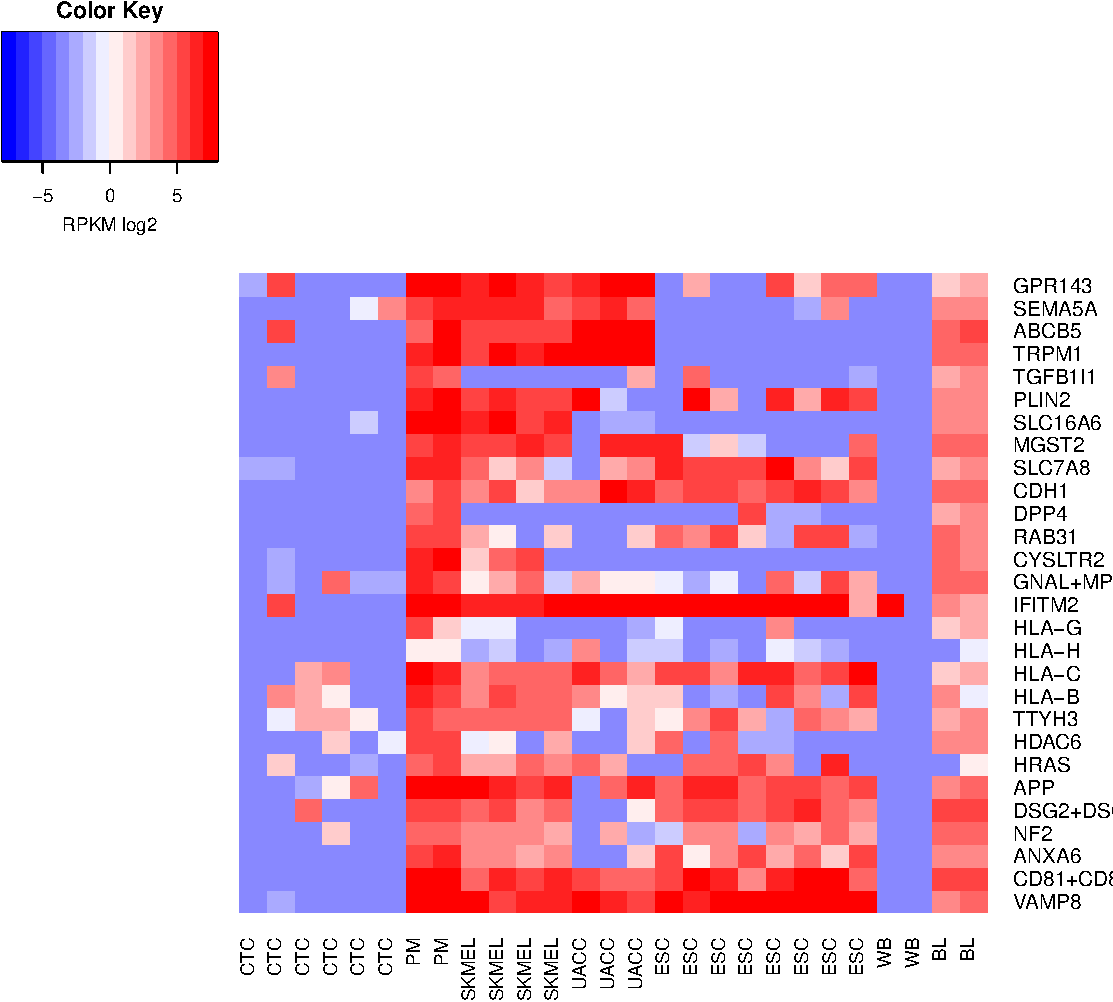
\includegraphics{Project_jankauskaite_ugne_files/figure-latex/unnamed-chunk-43-1.pdf}

\subsection{Discussion}\label{discussion}

The main goal of this project was to apply methods learned during the
course and reproduce real research results. Quantitatively, results were
not always exactly matching those of the selected paper (PCA analysis
for 12 cancer single sell samples, exact number of differentially
expressed genes between pairs of samples). This, among other reasons,
might happen due to updated reference files I used for alignment and
counting reads. Some small differences might also happen because of
different shift value when taking a logarithm. However, with one
exception the qualitative results of the original paper and this study
were the same. The reason of different qualitative results in expression
data heatmap of nine plasma membrane associated genes is unclear as the
exact numbers provided by authors in \textbf{supplementary table 4}
agree with the expression data obtained by this study.\\
Furthermore, in the future I would prefer using a different read counts
expression than RPKM. Doing the research for this project, I found that
RPKM were criticized by many researchers, see, for example Wagner, Kin,
and Lynch (2012). Also, it would be interesting to apply negative
binomial based models to the same raw counts data.

\section*{References}\label{references}
\addcontentsline{toc}{section}{References}

\hypertarget{refs}{}
\hypertarget{ref-plaks2013circulating}{}
Plaks, Vicki, Charlotte D Koopman, and Zena Werb. 2013. ``Circulating
Tumor Cells.'' \emph{Science} 341 (6151). American Association for the
Advancement of Science: 1186--8.

\hypertarget{ref-ramskold2012full}{}
Ramsköld, Daniel, Shujun Luo, Yu-Chieh Wang, Robin Li, Qiaolin Deng,
Omid R Faridani, Gregory A Daniels, et al. 2012. ``Full-Length mRNA-Seq
from Single-Cell Levels of Rna and Individual Circulating Tumor Cells.''
\emph{Nature Biotechnology} 30 (8). Nature Research: 777--82.

\hypertarget{ref-wagner2012measurement}{}
Wagner, Günter P, Koryu Kin, and Vincent J Lynch. 2012. ``Measurement of
mRNA Abundance Using Rna-Seq Data: RPKM Measure Is Inconsistent Among
Samples.'' \emph{Theory in Biosciences} 131 (4). Springer: 281--85.


\end{document}
